\documentclass[12pt,a4paper]{report}

% Packages
\usepackage{setspace}           % Line spacing
\usepackage[a4paper, left=1.5in, right=1in, top=1in, bottom=1in]{geometry}
\usepackage{titlesec}           % Chapter/section formatting
\usepackage{fancyhdr}           % Header/Footer
\usepackage{graphicx}           % Figures
\usepackage[hidelinks]{hyperref}  % Hyperlinks
\usepackage{tocloft}            % TOC formatting
\usepackage{etoolbox}
\usepackage{amsmath}
\usepackage{newtxtext}          % Times New Roman (text)
\usepackage{newtxmath}          % Times New Roman (mathematics)
\renewcommand{\texttt}[1]{\textrm{#1}}  % keep code-like words in Times as well
\renewcommand{\labelitemi}{$\bullet$}
\usepackage{booktabs}
\usepackage{longtable}
\usepackage{array}
\usepackage{float}
\usepackage{tikz}
\usetikzlibrary{arrows.meta,positioning,shapes.geometric,fit}
\usepackage{algorithm}
\usepackage{algpseudocode}
\usepackage{caption}
\usepackage{enumitem}
\usepackage[section]{placeins}  % keep figures and tables inside their own section
\usepackage{needspace}
\newcolumntype{L}[1]{>{\raggedright\arraybackslash}p{#1}}
\captionsetup{font=small, labelfont=bf, labelsep=colon, justification=centering}
\captionsetup[table]{position=top, skip=6pt}
\setlist{itemsep=3pt, topsep=4pt, parsep=0pt}
\setlength{\parskip}{6pt}
\renewcommand{\arraystretch}{1.25}

% Line spacing
\onehalfspacing

% Title formatting
\titleformat{\chapter}[display]{\bfseries\centering\LARGE}{Chapter \thechapter}{10pt}{}
\titleformat{\section}[hang]{\bfseries\Large}{\thesection}{1em}{}
\titleformat{\subsection}[hang]{\bfseries\large}{\thesubsection}{1em}{}
\titlespacing*{\chapter}{0pt}{0pt}{24pt}
\titlespacing*{\section}{0pt}{14pt}{8pt}
\titlespacing*{\subsection}{0pt}{10pt}{6pt}
% never leave a heading alone at the bottom of a page
\pretocmd{\section}{\Needspace*{7\baselineskip}}{}{}
\pretocmd{\subsection}{\Needspace*{5\baselineskip}}{}{}

% Fancy Header/Footer
\pagestyle{fancy}
\setlength{\headheight}{14.5pt}
\fancyhf{}
\lhead{\textit{ScamGuard: AI-Based Online Scam and Fraud Detection System}}
\lfoot{\textit{Dept. of CSE,BMSCE}}
\rfoot{\textit{Page \thepage}}

% Make chapter pages use fancy style
\makeatletter
\let\ps@plain\ps@fancy
\makeatother

\begin{document}

% ---------- FRONT MATTER: ROMAN NUMBERS ----------
\pagenumbering{roman}
\setcounter{page}{1}

% ----- Title Page -----
\begin{titlepage}
  \thispagestyle{empty}
  \centering

  {\Huge \textbf{ScamGuard: AI-Based Online Scam}}\\[0.25cm]{\Huge \textbf{and Fraud Detection System}}\\[1.0cm]
  
\includegraphics[width=0.18\linewidth]{VTU-Logojpg.jpg}\\[0.9cm]
  {\Large \textbf{PROJECT REPORT}}\\[0.2cm]
  {\large \textit{Submitted by}}\\[0.5cm]
  {\large Bhavya Goyal (1BM23CS063)}\\
  {\large Priyam Thakur (1BM23CS252)}\\
  {\large Samir Chaudhary (1BM23CS294)}\\
  {\large Sana Subodh (1BM23CS296)}\\[0.7cm]
  {\itshape in partial fulfillment for the award of the degree of}\\[0.15cm]
  {\Large \textbf{BACHELOR OF ENGINEERING}}\\[0.2cm]
  {\large in}\\[0.2cm]
  {\Large \textbf{COMPUTER SCIENCE AND ENGINEERING}}\\[0.9cm]
  {\large Under the Guidance of}\\
  {\large \textbf{Dr. Kayarvizhy N}}\\
  {\large Professor, Department of CSE, BMSCE}
  \vfill
  
\includegraphics[width=0.18\linewidth]{bmscelogo.jpg}\\[0.5cm]
  {\Large \textbf{B.M.S. COLLEGE OF ENGINEERING}}\\
  {\large (Autonomous Institution under VTU)}\\
  {\large BENGALURU - 560019}\\
  {\large Academic Year - 2026--2027}

\end{titlepage}
% ----- Certificate -----
\chapter*{Certificate}
\thispagestyle{empty}
\vspace{2cm}
This is to certify that the project report entitled \textbf{``ScamGuard: AI-Based Online Scam and Fraud Detection System''} is a bonafide work carried out by \textbf{Bhavya Goyal (USN: 1BM23CS063)}, \textbf{Priyam Thakur (USN: 1BM23CS252)}, \textbf{Samir Chaudhary (USN: 1BM23CS294)} and \textbf{Sana Subodh (USN: 1BM23CS296)} in partial fulfillment of the requirements for the award of the degree of \textbf{Bachelor of Engineering} in \textbf{Computer Science and Engineering}, under my supervision during the academic year 2026--2027.

\vspace{2cm}
\begin{flushleft}
Guide Signature\hspace{30mm} HoD signature \hspace{25mm} Principal Signature\\
(Dr. Kayarvizhy N) \hspace{22mm} Dr. Kavitha Sooda \hspace{19mm} Dr. Bheemsha Arya
\end{flushleft}
\vspace{2cm}
\begin{flushleft}
Name and signature of Examiners along with date \\
\vspace {1cm}
Examiner 1 \\
\vspace {1cm}
Examiner 2 \\
\end{flushleft}

% ----- Abstract -----
\chapter*{Abstract}
\thispagestyle{empty}
Fraudulent SMS messages are one of the cheapest ways to reach a phone user in India. They imitate bank KYC reminders, electricity disconnection notices, parcel delivery updates, traffic challans and job offers, and they increasingly arrive in Hindi or in a mix of Hindi and English. Public smishing collections contain only the messages that users chose to report, so they offer no verified genuine class, and a detector trained on them learns to distrust every bank-like message. ScamGuard was built to separate Indian scam messages from genuine ones with few false alarms and to explain each verdict.

We built ScamGuard-IN-2026, a corpus of 11,399 messages assembled from the India-relevant part of a 2025 research collection of user-reported smishing, a public set of real Indian SMS, scam texts quoted in 2025--26 government advisories and news reports, and synthetic messages that cover the newest scam types and are used for training only. Reported messages are not automatically scams, so we checked all 2,922 groups of near-identical reported messages, by rule or by reading them. About one in five retained reports turned out to be a genuine bank alert, OTP message, order update or advertisement. Messages were grouped into near-duplicate campaigns with MinHash, and the data was split so that no campaign appears in both training and testing.

The detector is a logistic-regression classifier over word and character TF-IDF features, combined with 31 interpretable intent patterns that explain each verdict by highlighting the exact phrases that make a message risky. On 1,874 held-out real messages from unseen campaigns, the classifier reaches an F1-score of 98.1\% with a 2.6\% false-alarm rate, and the deployed system reaches 97.1\% accuracy (95\% confidence interval 96.3--97.8\%) with a 3.2\% false-alarm rate. Training on unverified report labels instead of audited labels raises the false-alarm rate to 34.0\%. The detector is part of a working web application with a FastAPI back end and a Next.js front end, which offers a quick check without sign-in, a full analysis with phrase-level explanations, an AI copilot, safety tools for QR codes, UPI requests and files, scan history and analytics. The application is deployed on Render, and every number in this report can be reproduced from the project repository.

\vspace{0.4cm}\noindent\textbf{Keywords:} scam detection, smishing, SMS fraud, machine learning, natural language processing, label noise, data leakage, explainable AI

%-------------Declaration ----------
\chapter*{DECLARATION}
\thispagestyle{empty}
We hereby declare that the Major Project Phase-2 work entitled ``ScamGuard: AI-Based Online Scam and Fraud Detection System'' is a bonafide work and has been carried out by us under the guidance of Dr. Kayarvizhy N, Professor, Department of Computer Science and Engineering, B.M.S. College of Engineering, Bengaluru, in partial fulfillment of the requirements of the degree of Bachelor of Engineering in Computer Science and Engineering of Visvesvaraya Technological University, Belagavi.
We further declare that, to the best of our knowledge and belief, this project has not been submitted either in part or in full to any other university for the award of any degree.
\vspace{0.3cm}
\begin{flushleft}
Candidate details:
\end{flushleft}
\vspace{0.1cm}
\begin{center}
\begin{tabular}{|c|l|c|c|}
\hline
\textbf{SL. NO.} & \textbf{Student Name} & \textbf{USN} & \textbf{Student's Signature} \\
\hline
1 & Bhavya Goyal & 1BM23CS063 & \\
\hline
2 & Priyam Thakur & 1BM23CS252 & \\
\hline
3 & Samir Chaudhary & 1BM23CS294 & \\
\hline
4 & Sana Subodh & 1BM23CS296 & \\
\hline
\end{tabular}
\end{center}
\begin{flushleft}
Place: Bengaluru \\
Date: \\
\end{flushleft}
Certified that these candidates are students of Computer Science and Engineering Department of B.M.S. College of Engineering. They have carried out the project work titled ``ScamGuard: AI-Based Online Scam and Fraud Detection System'' as Major Project Phase-2 work. It is in partial fulfillment for completing the requirement for the award of B.E. degree by VTU. The work is original and we duly certify the same.
\vspace{1cm}
\begin{flushleft}
Guide Name: Dr. Kayarvizhy N\\
Date: \\
Signature \\
\end{flushleft}
% ----- Acknowledgment -----
\chapter*{Acknowledgment}
\thispagestyle{empty}
We are grateful to our guide, Dr. Kayarvizhy N, Professor, Department of Computer Science and Engineering, for steering this project towards a question that could be answered with evidence, and for insisting that the dataset reflect the messages people in India actually receive today. Her guidance on building a dataset that reflects current Indian scams shaped the audited corpus described here.

We thank Dr. Kavitha Sooda, Head of the Department of Computer Science and Engineering, and Dr. Bheemsha Arya, Principal, B.M.S. College of Engineering, for the facilities and the academic environment that made this work possible. We also thank the faculty members who reviewed our phase presentations and pointed out gaps in our evaluation.

We acknowledge the researchers who released the IMC 2025 smishing collection and the India Spam SMS collection under open licences; without them this study would have needed far more data collection. Finally, we thank our families and friends, several of whom forwarded the suspicious messages that shaped our test cases.
\newpage
% ----- TOC, LoF, LoT -----
\tableofcontents
\thispagestyle{empty}
\newpage
\listoffigures
\thispagestyle{empty}
\newpage
\listoftables
\thispagestyle{empty}

% ---------- MAIN MATTER: ARABIC NUMBERS ----------
\clearpage
\pagenumbering{arabic}
\setcounter{page}{1}

% ======================================================================
\chapter{Introduction}

\section{Overview}
A scam SMS rarely looks like a scam. It looks like a message from a bank asking for a quick KYC update, from an electricity board warning of disconnection tonight, from a courier holding a parcel for a small fee, or from the traffic police with a challan to pay through an attached app. Fraudsters copy the format of genuine service messages because people have learned to trust those formats. A detector has to tell the two apart even though they share most of their vocabulary: both mention OTPs, accounts, KYC, links and deadlines.

ScamGuard is a web application that does this for a single message pasted by the user. It returns a verdict, a risk score and, more importantly, the reasons: the phrases that make the message risky, the stage of the scam each phrase belongs to, what a genuine message from the same organisation would do instead, and what the user should do next. Behind the application is a text classifier and a layer of interpretable rules, both trained and evaluated on a dataset that we built for Indian messages.

This report describes the problem, the dataset, the detection method, the application and the evaluation. The research part of the project is also written up as a separate paper.

\section{Motivation}
Three observations motivated the project.

First, the scale and the Indian focus of the problem. A 2025 measurement study of more than 64,000 public smishing reports found that most attributable sender numbers belonged to Indian mobile operators~\cite{agarwal2025fishing}. The common Indian scams are well documented in advisories, but users still have to judge each message on their own.

Second, the cost of false alarms. Genuine Indian bank alerts, OTP messages and operator notices use the same words as scams: \textit{account}, \textit{KYC}, \textit{block}, \textit{OTP}, \textit{link}. Public smishing data contains only reported messages, and many of those reports are themselves genuine messages. A tool that cries wolf on real bank messages does damage, because it teaches users to ignore warnings.

Third, the lack of explanation in most tools. A bare ``spam'' label gives the user nothing to act on. Users need to see which part of the message is the trap, so that they can recognise the next one without a tool.

\section{Objective}
The objectives of the project are:
\begin{enumerate}
\item To build a labelled dataset of Indian scam and genuine SMS that reflects current scam types and whose labels have been checked, rather than taken from user reports at face value.
\item To evaluate lightweight text classifiers on that dataset under a protocol that prevents near-duplicate messages from leaking between training and testing.
\item To combine the best classifier with interpretable intent rules that explain each verdict at phrase level, and to measure honestly whether the rules also improve accuracy.
\item To deliver the detector in a usable, deployed web application with supporting safety tools, history and analytics.
\item To make every reported result reproducible from the project repository.
\end{enumerate}

\section{Scope}
The system analyses one message at a time, as pasted by the user, in English, Hindi (Devanagari script) or romanised Hindi. It classifies the message as \emph{scam} or \emph{legitimate}. A scam is a message that tries to obtain money, a secret such as an OTP or PIN, personal data, an app installation or a call to a private number by deception. Genuine advertisements are legitimate. The application also accepts URLs, e-mails, screenshots, PDFs and QR codes, which it converts to text or checks with separate tools.

The project does not intercept messages on the phone, does not use sender metadata or conversation history in the classifier, and does not cover Indian languages other than Hindi. The risk score is a ranking signal, not a calibrated probability, and the verdict is advice, not proof of fraud.

\section{SDG Justification}
The project addresses the following United Nations Sustainable Development Goals.
\begin{itemize}
\item \textbf{SDG 16 (Peace, Justice and Strong Institutions), target 16.4 on reducing illicit financial flows.} Scam messages are the entry point of many financial frauds. Helping users recognise them before they pay or share an OTP reduces the money that reaches fraudsters, and the application points users to the official reporting channels (helpline 1930 and cybercrime.gov.in).
\item \textbf{SDG 8 (Decent Work and Economic Growth), target 8.10 on access to financial services.} Digital payments only widen financial access if people can trust them. A tool that separates genuine bank and UPI messages from imitations supports that trust, especially for first-time digital users.
\item \textbf{SDG 9 (Industry, Innovation and Infrastructure), target 9.c on access to ICT.} The detector is small enough to run on free cloud infrastructure and answers in milliseconds, so it can be offered at no cost to users.
\item \textbf{SDG 10 (Reduced Inequalities).} Support for Hindi messages and a simplified ``elder mode'' interface aim at users who are most often targeted and least served by English-only tools.
\end{itemize}

\section{Existing System}
Existing approaches fall into three groups.
\begin{itemize}
\item \textbf{Operator and regulator measures.} Telecom operators filter bulk traffic and register commercial senders, and users can report unwanted messages to the 1909 DND service or to the cyber-crime portal. These measures act on senders and volumes; they do not help a user judge a message that has already arrived from an ordinary mobile number.
\item \textbf{Rule-based and keyword filters.} Phone apps and simple filters flag words such as ``lottery'' or ``KYC''. They are easy to explain but flag many genuine messages that use the same words and miss scams that avoid them.
\item \textbf{Machine-learning filters in research.} Classifiers such as Naive Bayes, SVM, CNN and LSTM report high accuracy, but mostly on promotional spam, with random train-test splits and without a genuine Indian class~\cite{almeida2013towards,roy2020deep,goel2024ml}. Newer report-based corpora contain only reported messages~\cite{timko2024smishing,agarwal2025fishing}.
\end{itemize}

\section{Proposed System}
The proposed system has three parts.
\begin{enumerate}
\item \textbf{A dataset, ScamGuard-IN-2026.} Real Indian reported scams, real Indian genuine messages, 2025--26 advisory texts and synthetic messages for the newest scam types, with every reported-message group checked and the data split by scam campaign.
\item \textbf{A detector.} Logistic regression over word and character TF-IDF features, which handles Hindi and obfuscated spellings, combined with interpretable intent rules and genuine-message guards that explain each verdict.
\item \textbf{A complete application.} A deployed web application with a quick check, a full analysis with Scam X-Ray and TrustLens explanations, an AI copilot, safety tools, history, analytics and an automated daily check of the live site.
\end{enumerate}

\section{Work Plan}
Table~\ref{tab:workplan} shows the work plan across the two project phases.

\begin{table}[H]
\centering
\caption{Work plan}
\label{tab:workplan}
\begin{tabular}{|L{1.3cm}|L{5cm}|L{6.8cm}|}
\hline
\textbf{Phase} & \textbf{Activity} & \textbf{Outcome} \\
\hline
1 & Problem study and literature survey & Research gap: no verified Indian genuine class, leakage-prone evaluation \\
\hline
1 & Requirement analysis and design & System architecture, data model and user flows \\
\hline
1 & Application architecture & FastAPI back end, Next.js front end, model registry, database \\
\hline
2 & Explanation layer & Intent rules, Scam X-Ray, TrustLens, retrieval of known patterns \\
\hline
2 & Dataset construction & ScamGuard-IN-2026 with label audit and campaign split \\
\hline
2 & Model selection and experiments & Final model; leakage, label-audit, training-data and fusion experiments \\
\hline
2 & Deployment and testing & Render deployment, 818 automated tests, daily live-site check \\
\hline
2 & Documentation & Report, research paper, presentation \\
\hline
\end{tabular}
\end{table}

% ======================================================================
\chapter{Literature Survey}

\section{Overview}
We reviewed work on SMS spam corpora, smishing detection, report-based measurement studies and general machine-learning methodology for label noise and data leakage. Each reference below was checked against its publisher page, DOI record or arXiv entry. Results quoted are those stated by the authors; where a value is not stated we say so.

\section{Detailed Survey}

\textbf{SMS Spam Collection.} Almeida, G\'omez Hidalgo and Yamakami released the SMS Spam Collection in 2011~\cite{almeida2011contributions}: 5,574 English messages, 747 of them spam, mostly from the UK. In a follow-up they compared many classifiers and tokenisers and preferred a linear SVM, which reached 97.64\% accuracy while blocking only 0.18\% of legitimate messages~\cite{almeida2013towards}. The corpus is clean and public, which explains its popularity, but its positive class consists of prize draws and ringtone offers rather than the scams we target.

\textbf{Deep learning on the same corpus.} Roy, Singh and Banerjee trained CNN and LSTM models on the corpus and reported up to 99.44\% accuracy~\cite{roy2020deep}. Ahmadi \textit{et al.} compared six classifiers with TF-IDF and bag-of-words features on a Kaggle copy and reported accuracies between 0.91 and 0.95, although some values in their text and tables disagree~\cite{ahmadi2025llm}. Labonne and Moran showed that a fine-tuned Flan-T5 model beats classical baselines for e-mail spam, especially with little training data~\cite{labonne2023spamt5}.

\textbf{Smishing detection.} Sonowal and Kuppusamy proposed SmiDCA, which selects content features for machine-learning anti-smishing classifiers~\cite{sonowal2018smidca}. Mishra and Soni combined SMS content analysis with the behaviour of embedded URLs and reported 96.29\% accuracy~\cite{mishra2020smishing}. Goel \textit{et al.} extracted smishing messages from the SMS Spam Collection, added 71 web messages, normalised slang and trained Naive Bayes, reaching 96.2\% accuracy and a 3.87\% false-positive rate~\cite{goel2024ml}.

\textbf{Report-based corpora.} Timko and Rahman released 1,062 validated Smishtank submissions with URL and sender metadata~\cite{timko2024smishing}. Agarwal \textit{et al.} mined five public forums from 2017 to 2024, labelled scam type, brand and lure with GPT-4o, and released 33,869 labelled messages in 66 languages~\cite{agarwal2025fishing}. They state that user reports carry no verification. The same group analysed 1.2 million UK operator reports from 2024 and found that 35.12\% of unique reported texts were spam rather than scams~\cite{agarwal2026overview}. MOZ-Smishing provides labelled genuine and fraudulent mobile-money messages for Mozambique~\cite{ali2025moz}.

\textbf{Surveys.} Pritom \textit{et al.} reviewed 119 smishing papers and found datasets ``often limited in scale, diversity, and temporal coverage'', along with imbalanced data, synthetic evaluation data and subjective labelling of non-spam messages~\cite{pritom2026sms}.

\textbf{Methodology.} Northcutt, Jiang and Chuang showed that disagreements between cross-validated predictions and given labels locate many label errors (confident learning)~\cite{northcutt2021confident}. Lee \textit{et al.} showed that near-duplicates inflate evaluation of language models, with train-test overlap in over 4\% of standard validation sets~\cite{lee2022dedup}. Kapoor and Narayanan list duplicate data across train and test among the most common leakage errors in applied machine learning~\cite{kapoor2023leakage}. MinHash, introduced by Broder~\cite{broder1997resemblance}, is the standard tool for finding near-duplicate documents at scale.

Table~\ref{tab:lit} summarises the most relevant studies.

{\small
\renewcommand{\arraystretch}{1.1}
\begin{longtable}{|L{2.1cm}|L{2.6cm}|L{2.8cm}|L{2.2cm}|L{2.7cm}|}
\caption{Summary of related work}\label{tab:lit}\\
\hline
\textbf{Work} & \textbf{Technique} & \textbf{Dataset} & \textbf{Reported result} & \textbf{Limitation for our problem} \\
\hline
\endfirsthead
\hline
\textbf{Work} & \textbf{Technique} & \textbf{Dataset} & \textbf{Reported result} & \textbf{Limitation for our problem} \\
\hline
\endhead
Almeida \textit{et al.}, 2013~\cite{almeida2013towards} & Many classifiers; linear SVM preferred & SMS Spam Collection, UK, 5,574 & 97.64\% acc., 0.18\% ham blocked & Promotional spam, not Indian scams \\
\hline
Roy \textit{et al.}, 2020~\cite{roy2020deep} & CNN, LSTM & Same corpus & 99.44\% acc. & Same corpus, no cross-domain test \\
\hline
Mishra, Soni, 2020~\cite{mishra2020smishing} & Content + URL behaviour & SMS datasets & 96.29\% acc. & Depends on URLs \\
\hline
Goel \textit{et al.}, 2024~\cite{goel2024ml} & Slang normalisation + Naive Bayes & Public smishing subset + 71 web messages & 96.2\% acc., FPR 3.87\% & 362 smishing messages \\
\hline
Timko, Rahman, 2024~\cite{timko2024smishing} & Data release & Smishtank, 1,062 & No classifier & No genuine class \\
\hline
Agarwal \textit{et al.}, 2025~\cite{agarwal2025fishing} & GPT-4o labelling & 33,869 reports & No classifier & Reports unverified; no genuine class \\
\hline
Pritom \textit{et al.}, 2026~\cite{pritom2026sms} & Systematic review & 119 papers & Not applicable & Identifies the dataset gap \\
\hline
\end{longtable}}


\section{Research Gap Identification}
The survey points to four gaps.
\begin{enumerate}
\item \textbf{No verified genuine Indian class.} Classical corpora are not Indian; report-based corpora contain only reported messages. No public resource pairs Indian scams with Indian genuine messages under checked labels.
\item \textbf{Report labels are taken at face value.} Report-based corpora are used as if every report were a scam, although their own authors warn that reports are unverified and the UK study found large fractions of spam and OTPs among reports.
\item \textbf{Evaluation ignores campaigns.} Scam campaigns repeat one template many times. Random splits put copies of the same template on both sides, which inflates results, and none of the surveyed SMS studies controls for this.
\item \textbf{Explanation and rules are not evaluated independently.} Hybrid systems add rules, but their benefit is usually measured on messages chosen by the same developers.
\end{enumerate}

\section{Mapping of Objectives with Research Gap Identification}
\begin{table}[H]
\centering
\caption{Mapping of objectives to research gaps}
\label{tab:mapping}
\begin{tabular}{|L{6.3cm}|L{7.2cm}|}
\hline
\textbf{Objective} & \textbf{Gap addressed} \\
\hline
1. Build an Indian dataset with checked labels & Gaps 1 and 2: genuine Indian class; audit of report labels \\
\hline
2. Evaluate under a leakage-free protocol & Gap 3: campaign-aware split \\
\hline
3. Combine classifier with interpretable rules and measure their value & Gap 4: rules evaluated on independent real data \\
\hline
4. Deliver a deployed application & Practical use of the findings \\
\hline
5. Reproducibility & Supports verification of all four gaps \\
\hline
\end{tabular}
\end{table}

% ======================================================================
\chapter{Software and Hardware Requirement Specification}

\section{Functional Requirements}
\begin{enumerate}
\item \textbf{Quick check.} A visitor can paste a message on the home page and receive a verdict, risk score, highlighted trap phrases and a short explanation without creating an account.
\item \textbf{Account management.} Users can register and sign in (with a captcha), or open a demo account, and can update or delete their profile and export their data.
\item \textbf{Full analysis.} A signed-in user can analyse text, a URL, an e-mail, a screenshot, a PDF or a QR code. The result includes the verdict, the classifier probability, the final risk score, the Scam X-Ray stages, the TrustLens report and recommended actions.
\item \textbf{Explanation.} For each result the system shows the matched phrases with their scam stage (hook, pressure, request, cash-out), evidence for and against, a similar known pattern with its source when one is accepted by the retrieval evaluator, and how a genuine message would differ.
\item \textbf{AI copilot.} Users can ask follow-up questions in English or Hindi; answers come from a hosted language model with per-visitor and daily limits, and fall back to built-in answers when the limit is reached.
\item \textbf{Safety tools.} QR code check, a ``before you pay'' check for UPI requests, a file check that detects disguised Android apps, a what-if view that shows how each cue changes the score, and a chat timeline that finds the turning point of a conversation.
\item \textbf{History, cases and reports.} Users can browse and search past scans, group scans into investigation cases with notes, give feedback on verdicts, download a PDF report and report a scam to the community view.
\item \textbf{Analytics.} Users see totals, verdict share and score trends; a public page shows aggregated scam trends.
\item \textbf{Administration.} Administrators can view registered model versions and their metrics and run a robustness test.
\end{enumerate}

\section{Non-functional Requirements}
\begin{itemize}
\item \textbf{Performance.} Classification of one message takes about 2~ms, and about 4~ms including the intent layer, on a two-core server; page responses are compressed and cached.
\item \textbf{Reliability.} The model is loaded once at start-up from a versioned registry; if the configured database is unreachable, the service starts on a local fallback database instead of failing. An automated job checks the live site every morning.
\item \textbf{Security.} Passwords are hashed, access uses signed tokens with refresh, endpoints are rate-limited, request bodies are size-limited, and security headers are set.
\item \textbf{Privacy.} The quick check stores nothing, and contributed messages are masked before they are stored.
\item \textbf{Usability.} English and Hindi interface, an elder mode with larger text, keyboard-accessible controls, and layouts that work at phone width.
\item \textbf{Maintainability.} Training and serving share the same preprocessing code; 818 automated back-end and ML tests run on every change.
\end{itemize}

\section{Hardware Requirements}
\begin{table}[H]
\centering
\caption{Hardware requirements}
\begin{tabular}{|L{4cm}|L{9.5cm}|}
\hline
\textbf{Component} & \textbf{Requirement} \\
\hline
Development machine & Any laptop with 8~GB RAM and a recent 64-bit CPU; no GPU is needed \\
\hline
Training & Under 3 seconds for the production model on a two-core CPU \\
\hline
Server & One small cloud instance (512~MB RAM is sufficient for the model, 1.6~MB on disk) \\
\hline
Client & Any browser on a phone or computer \\
\hline
\end{tabular}
\end{table}

\section{Software Requirements}
\begin{table}[H]
\centering
\caption{Software requirements}
\begin{tabular}{|L{4cm}|L{9.5cm}|}
\hline
\textbf{Layer} & \textbf{Software} \\
\hline
Language & Python 3.10+ (tested on 3.13), TypeScript 5.5 \\
\hline
Machine learning & scikit-learn 1.7, NumPy, pandas, SciPy, joblib, datasketch (dataset build), matplotlib (figures) \\
\hline
Back end & FastAPI 0.115, Uvicorn, SQLAlchemy 2.0, Alembic, Pydantic 2, SlowAPI, python-jose, passlib, ReportLab, Tesseract OCR \\
\hline
Front end & Next.js 14.2, React 18.3, Tailwind CSS 3.4, Recharts, Zod, Vitest \\
\hline
Database & PostgreSQL in production, SQLite locally \\
\hline
Deployment & Render (back end and front end), GitHub Actions for CI and the daily live check \\
\hline
Language model & Google Gemini through its API for the copilot (optional) \\
\hline
\end{tabular}
\end{table}

\section{Cost Estimation}
The project was built and deployed with free resources. Development used the team's own laptops. The application runs on Render's free tier, the copilot uses a free API tier with a daily request cap, and all libraries are open source. The datasets are free to use under their CC BY 4.0 and MIT licences. The recurring cost of the deployed prototype is therefore zero. A production deployment for many users would need a paid always-on instance and a managed database, priced according to the provider's current plans.

% ======================================================================
\chapter{Methodology}

\section{Tools and Techniques}
\begin{itemize}
\item \textbf{TF-IDF} weights a term by how often it occurs in a message and how rare it is across messages~\cite{salton1988term}. We use word unigrams and bigrams together with character 2--5-grams.
\item \textbf{Logistic regression} gives a linear, interpretable model whose coefficients show which words push a message towards ``scam''.
\item \textbf{MinHash with locality-sensitive hashing}~\cite{broder1997resemblance} groups near-identical messages into campaigns.
\item \textbf{Confident learning}~\cite{northcutt2021confident} guides a second review of labels that a cross-validated model contradicts.
\item \textbf{Regular-expression intent rules} detect requests for OTPs, payments to receive money, remote-access apps, legal threats and similar tactics, and protective signals such as ``do not share your OTP''.
\item \textbf{Bootstrap confidence intervals and McNemar's test} quantify uncertainty and compare models on the same messages.
\item \textbf{scikit-learn}~\cite{pedregosa2011scikit} implements the models; FastAPI and Next.js implement the application.
\end{itemize}

\section{Data Set With Explanation}

\subsection{Need for an Indian dataset}
Indian scam messages and Indian genuine service messages share most of their vocabulary, and public smishing data contains only reported messages with unverified labels. A detector for Indian users therefore needs real Indian genuine messages, checked labels for reported messages and current scam types. ScamGuard-IN-2026 was built for this purpose, and it is the only dataset used for training and evaluation in this project.

\subsection{Sources}
\begin{table}[H]
\centering
\caption{Sources of ScamGuard-IN-2026}
\label{tab:sources}
\small
\begin{tabular}{|L{3.6cm}|L{2.1cm}|L{1.4cm}|L{1.2cm}|L{3.6cm}|}
\hline
\textbf{Source} & \textbf{Licence} & \textbf{Genuine} & \textbf{Scam} & \textbf{Use} \\
\hline
R1: IMC 2025 smishing collection, India subset, audited~\cite{agarwal2025fishing} & CC BY 4.0 & 963 & 3,987 & train, development, test \\
\hline
R2: India Spam SMS collection, audited & MIT & 1,694 & 6 & train, development, test \\
\hline
R3: 2025--26 advisory and news texts & Quoted with source & 1 & 11 & test only \\
\hline
R4: Team-contributed 2026 SMS, masked & Team consent & -- & -- & test only (being collected) \\
\hline
S: Synthetic templates & Project & 2,950 & 1,787 & training only \\
\hline
\textbf{Total} & & \textbf{5,608} & \textbf{5,791} & \textbf{11,399 messages} \\
\hline
\end{tabular}
\end{table}

\textbf{R1} is the part of the IMC 2025 collection that concerns India: English or Hindi messages whose sender network is Indian or whose text names an Indian bank, payment app, identity document, operator or currency. The collection's ``spam'' category, which holds advertisements, was excluded. \textbf{R2} contains Indian personal, work and promotional messages. \textbf{R3} holds twelve messages from 2025--26 advisories and news, stored with source URL and date, including one genuine operator notice from a team member's phone. \textbf{R4} will hold messages received by the team in 2026, masked for personal data. \textbf{S} covers scam types that are new or rare in the real data, such as digital arrest calls, e-challan and wedding-invitation APKs, task-based jobs, stock-tip groups, Hindi electricity threats and fake ``amount credited'' messages, and genuine Indian formats such as bank alerts, OTPs with warnings, delivery and ride codes, operator and government notices and personal chat. Synthetic messages are never used for testing.

\subsection{Attributes}
Each row of the dataset has seven attributes: \texttt{text} (the message), \texttt{label} (\texttt{scam} or \texttt{legitimate}), \texttt{source} (R1--R4 or synthetic), \texttt{subtype} (scam type or genuine type), \texttt{is\_synthetic}, \texttt{campaign} (near-duplicate group) and \texttt{split} (train, development, test or 2026 test).

\subsection{Label audit}
The IMC 2025 messages are messages that users \emph{reported}. When we read a sample, about a third of the groups were genuine. We therefore checked every group:
\begin{enumerate}
\item 1,253 groups had a strong fraud cue (an account threat plus a KYC or call instruction, a prize plus a fee, a request to share an OTP) and no genuine cue, and were confirmed as scams by rule. A spot check of 40 found no error.
\item The other 1,669 groups were read one by one: 583 were scams, 867 genuine and 219 unclear, which were dropped.
\item A cross-validated model then flagged 44 rows whose label it strongly contradicted; each was re-read, giving 19 corrections and 7 removals.
\end{enumerate}
After the audit, 963 of 4,950 retained IMC rows (19.5\%) are genuine: debit and credit alerts, OTP messages with a warning, shipping updates, premium reminders and bank advertisements. Six disguised scams were also found among the R2 promotions. Every decision is stored in audit files in the repository.

\subsection{Campaigns and splits}
Messages are grouped into campaigns when their MinHash-estimated Jaccard similarity over word 3-shingles is at least 0.6. The 6,662 real messages form 4,085 campaigns; the largest has 128 messages and the largest 1\% of campaigns hold 14\% of real messages. Each campaign goes entirely to training (60\%), development (15\%) or test (25\%), chosen by a hash of its first message. Table~\ref{tab:splits} gives the final counts.

\begin{table}[H]
\centering
\caption{Dataset splits}
\label{tab:splits}
\begin{tabular}{|l|r|r|l|}
\hline
\textbf{Split} & \textbf{Genuine} & \textbf{Scam} & \textbf{Content} \\
\hline
Train & 4,581 & 4,064 & real and synthetic \\
\hline
Development & 361 & 507 & real only \\
\hline
Test & 665 & 1,209 & real only, unseen campaigns \\
\hline
2026 test & 1 & 11 & advisories (team data pending) \\
\hline
\end{tabular}
\end{table}

\section{Flow Chart Of Methodology From Start To End}
Figure~\ref{fig:flow} shows the methodology from data collection to deployment, and Figure~\ref{fig:arch} the architecture of the deployed system.

\begin{figure}[H]
\centering
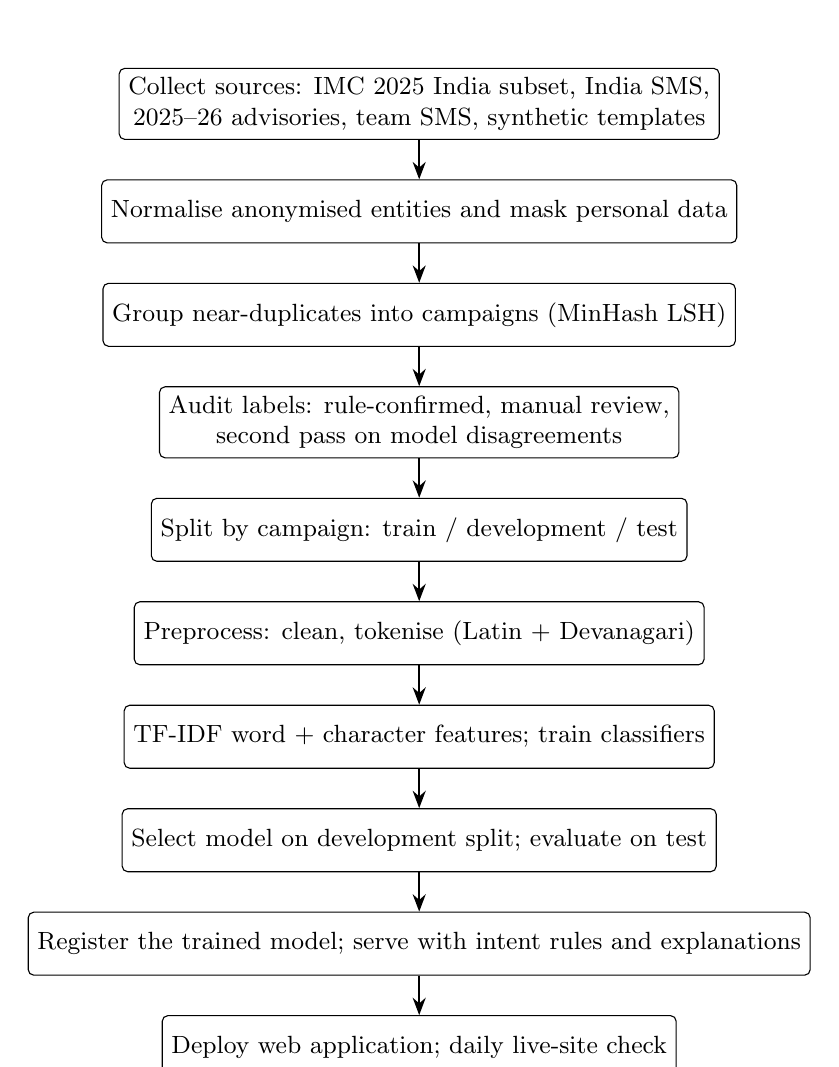
\begin{tikzpicture}[node distance=5mm,
  box/.style={draw, rounded corners=2pt, align=center, font=\small, minimum width=6.5cm, minimum height=8mm, fill=white},
  arr/.style={-{Stealth[length=2.2mm]}, thick}]
\node[box] (a) {Collect sources: IMC 2025 India subset, India SMS,\\2025--26 advisories, team SMS, synthetic templates};
\node[box, below=of a] (b) {Normalise anonymised entities and mask personal data};
\node[box, below=of b] (c) {Group near-duplicates into campaigns (MinHash LSH)};
\node[box, below=of c] (d) {Audit labels: rule-confirmed, manual review,\\second pass on model disagreements};
\node[box, below=of d] (e) {Split by campaign: train / development / test};
\node[box, below=of e] (f) {Preprocess: clean, tokenise (Latin + Devanagari)};
\node[box, below=of f] (g) {TF-IDF word + character features; train classifiers};
\node[box, below=of g] (h) {Select model on development split; evaluate on test};
\node[box, below=of h] (i) {Register the trained model; serve with intent rules and explanations};
\node[box, below=of i] (j) {Deploy web application; daily live-site check};
\foreach \x/\y in {a/b,b/c,c/d,d/e,e/f,f/g,g/h,h/i,i/j} \draw[arr] (\x) -- (\y);
\end{tikzpicture}
\caption{Flow of the methodology}
\label{fig:flow}
\end{figure}

\begin{figure}[H]
\centering
\resizebox{\linewidth}{!}{%
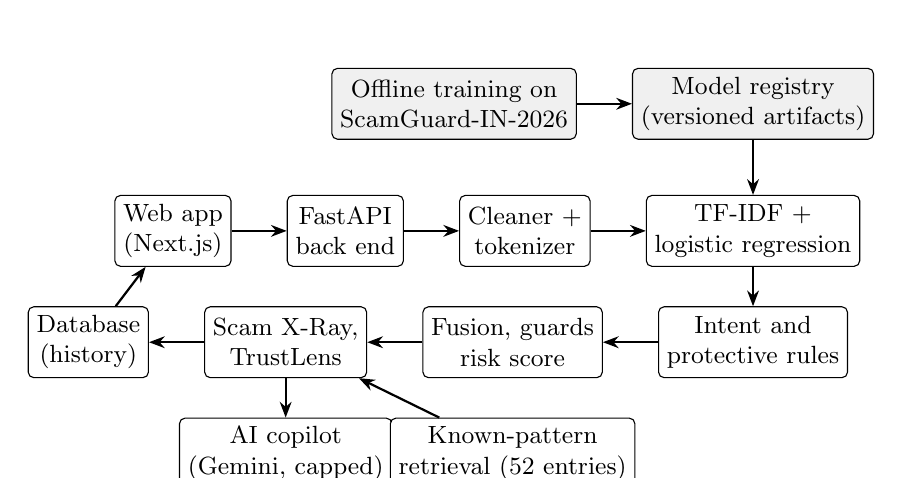
\begin{tikzpicture}[
  node distance=5mm and 7mm,
  box/.style={draw, rounded corners=2pt, align=center, font=\small, minimum height=9mm, inner sep=3pt, fill=white},
  off/.style={box, fill=gray!12},
  arr/.style={-{Stealth[length=2mm]}, thick}]
\node[box] (ui) {Web app\\(Next.js)};
\node[box, right=of ui] (api) {FastAPI\\back end};
\node[box, right=of api] (pre) {Cleaner +\\tokenizer};
\node[box, right=of pre] (clf) {TF-IDF +\\logistic regression};
\node[box, below=of clf] (rules) {Intent and\\protective rules};
\node[box, left=of rules] (fuse) {Fusion, guards\\risk score};
\node[box, left=of fuse] (expl) {Scam X-Ray,\\TrustLens};
\node[box, left=of expl] (db) {Database\\(history)};
\node[off, above=7mm of clf] (reg) {Model registry\\(versioned artifacts)};
\node[off, left=of reg] (train) {Offline training on\\ScamGuard-IN-2026};
\node[box, below=of expl] (cop) {AI copilot\\(Gemini, capped)};
\node[box, below=of fuse] (rag) {Known-pattern\\retrieval (52 entries)};
\draw[arr] (ui) -- (api); \draw[arr] (api) -- (pre); \draw[arr] (pre) -- (clf);
\draw[arr] (clf) -- (rules); \draw[arr] (rules) -- (fuse); \draw[arr] (fuse) -- (expl);
\draw[arr] (expl) -- (db); \draw[arr] (db) -- (ui);
\draw[arr] (train) -- (reg); \draw[arr] (reg) -- (clf);
\draw[arr] (rag) -- (expl); \draw[arr] (expl) -- (cop);
\end{tikzpicture}}
\caption{Architecture of the deployed system. Shaded parts run offline.}
\label{fig:arch}
\end{figure}

\section{Explanation Of Methodology In Details With Equations And Formulae}

\subsection{Problem definition}
For a message $x$, the detector computes a score $s(x)\in[0,1]$ and predicts
\begin{equation}
\hat{y}=\begin{cases}1 \;(\text{scam}) & \text{if } s(x)\ge 0.5\\ 0 \;(\text{legitimate}) & \text{otherwise.}\end{cases}
\end{equation}

\subsection{Preprocessing}
The cleaner replaces e-mail addresses, URLs (including bare links such as \texttt{bit.ly/x}) and phone numbers with placeholder tokens, lowercases the text, removes punctuation while keeping Devanagari vowel signs, and replaces remaining numbers with a number token. The tokenizer keeps Latin and Devanagari words, removes English stop words and applies a light suffix stemmer. The same code runs in training and in the live service, which rules out train-serve skew. Devanagari words are kept intact, so Hindi messages contribute features just as English ones do.

\subsection{Feature extraction}
For a term $t$ in message $d$, with $N$ training messages and document frequency $\mathrm{df}(t)$, the TF-IDF weight is
\begin{equation}
w_{t,d}=\left(1+\log \mathrm{tf}_{t,d}\right)\cdot\left(\log\frac{1+N}{1+\mathrm{df}(t)}+1\right),
\end{equation}
and each message vector is normalised to unit length. Word features use unigrams and bigrams (up to 30,000, minimum document frequency 2, maximum 95\%); character features use 2--5-grams inside word boundaries (up to 60,000, minimum document frequency 2). The two vectors are concatenated into $\phi(x)$ with 35,148 dimensions after pruning. Character n-grams let the model recognise \textit{K.Y.C}, \textit{bl0cked} or \textit{S I M} as the words they imitate.

\subsection{Classifier}
Logistic regression estimates
\begin{equation}
p(x)=\sigma\!\left(\mathbf{w}^{\top}\phi(x)+b\right)=\frac{1}{1+e^{-(\mathbf{w}^{\top}\phi(x)+b)}},
\end{equation}
by minimising the class-weighted, $\ell_2$-regularised log-loss
\begin{equation}
\min_{\mathbf{w},b}\;\frac{1}{2}\|\mathbf{w}\|^2 + C\sum_{i=1}^{n}\alpha_{y_i}\Big[-y_i\log p(x_i)-(1-y_i)\log\big(1-p(x_i)\big)\Big],
\end{equation}
with $C=16$ and class weights $\alpha_c=n/(2n_c)$. The per-word contribution to a verdict is $w_t\,w_{t,d}$, which the application shows as the classifier's top words.

\subsection{Intent evidence and fusion}
Thirty-one patterns detect 26 scam intents with hand-set weights $w_i$ and ten protective signals with weights $v_j$. With $E^{+}=\sum_{i\in I(x)}w_i$ (halved when only weak context cues match) and $E^{-}=\sum_{j\in P(x)}v_j$ (halved when $E^{+}\ge 0.5$), the final score is
\begin{equation}
s(x)=\sigma\!\Big(\operatorname{clip}\big(\operatorname{logit}p(x),-4,4\big)+5\,(E^{+}-E^{-})\Big),
\end{equation}
and it is capped at 0.15 when the message has the shape of a genuine transaction alert or service notice without any blocking cue (an install or payment request, a call to action on a credited amount, a private phone number). A ``decoy'' rule catches messages that say ``never share your OTP'' and then ask for it.

\subsection{Evaluation metrics}
With scam as the positive class:
\begin{align}
\text{Precision}&=\frac{TP}{TP+FP}, & \text{Recall}&=\frac{TP}{TP+FN},\\
F_1&=\frac{2\cdot\text{Precision}\cdot\text{Recall}}{\text{Precision}+\text{Recall}}, & \text{False-alarm rate}&=\frac{FP}{FP+TN}.
\end{align}
A false positive is a genuine message wrongly flagged, which is the error users notice first. Confidence intervals come from 1,000 bootstrap resamples, and paired comparisons use McNemar's test on the messages two models classify differently.

\subsection{Inference procedure}
\begin{algorithm}[H]
\caption{Scoring one message in the live service}
\begin{algorithmic}[1]
\Require message $x$; frozen vectorizer and model; intent rules
\State $t\gets$ \textsc{Tokenize}(\textsc{Clean}($x$))
\State $p\gets\sigma(\mathbf{w}^\top\phi(t)+b)$
\State find matched intents $I$ and protective signals $P$
\If{a sentence asks for an OTP after a ``never share'' warning} \State add decoy intent \EndIf
\State $s\gets\sigma(\operatorname{clip}(\operatorname{logit}p,\pm4)+5(E^+-E^-))$
\If{genuine alert or notice with no blocking cue} \State $s\gets\min(s,0.15)$ \EndIf
\State \Return verdict $\mathbf{1}[s\ge0.5]$, $p$, $s$, highlighted phrases, explanation
\end{algorithmic}
\end{algorithm}

% ======================================================================
\chapter{Results and Discussion}

\section{Experimental setup}
Models were selected on the development split and then trained on the training and development splits together (9,513 messages). All results below are on the real test split: 1,874 messages (665 genuine, 1,209 scams) from campaigns never seen in training. We also report a 259-message challenge set that the team wrote while designing the rules; because the same people wrote both, it is a development check, not an independent test. Experiments ran on a two-core Intel Xeon at 2.8~GHz with Python 3.13 and scikit-learn 1.7.2. One script produces every table.

\section{Performance of the deployed system}
Table~\ref{tab:final} and Figure~\ref{fig:final} give the main result: all metrics of the deployed system on the real test set, next to the classifier alone and the learned fusion weights described in Section~\ref{sec:fusionexp}.

\begin{table}[H]
\centering
\caption{Real test set, 1,874 messages from unseen campaigns (\%; FAR = false-alarm rate)}
\label{tab:final}
\begin{tabular}{|l|r|r|r|r|r|r|}
\hline
\textbf{System} & \textbf{Acc.} & \textbf{Prec.} & \textbf{Rec.} & \textbf{F1} & \textbf{FAR} & \textbf{AUC} \\
\hline
Classifier only & 97.5 & 98.6 & 97.6 & 98.1 & 2.6 & 0.997 \\
\hline
Deployed system (hand rules) & 97.1 & 98.2 & 97.2 & 97.7 & 3.2 & 0.995 \\
\hline
Learned fusion & \textbf{97.8} & \textbf{98.7} & \textbf{97.8} & \textbf{98.3} & \textbf{2.3} & 0.997 \\
\hline
\end{tabular}
\end{table}

The deployed system catches 1,175 of the 1,209 test scams and passes 644 of the 665 genuine messages. The 95\% confidence interval of its accuracy is 96.3--97.8\%, and of its false-alarm rate 2.0--4.6\%. On the twelve 2025--26 advisory messages it detects 10 of the 11 scams and passes the one genuine operator notice (F1 95.2\%); this set is too small for a firm conclusion.

\begin{figure}[H]
\centering
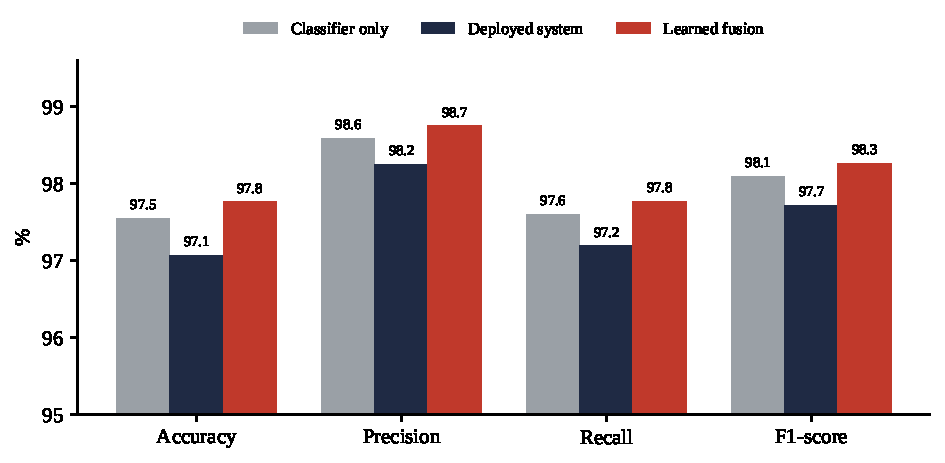
\includegraphics[width=0.62\linewidth]{figures/final_metrics.pdf}
\caption{Accuracy, precision, recall and F1-score on the real test set (vertical axis starts at 95\%)}
\label{fig:final}
\end{figure}



\section{Comparison of models and features}
\begin{table}[H]
\centering
\caption{Classifiers on the real test set (\%); ``Challenge'' is F1 on the 259 team-written messages}
\label{tab:models}
\begin{tabular}{|l|l|r|r|r|}
\hline
\textbf{Model} & \textbf{Features} & \textbf{F1} & \textbf{False alarms} & \textbf{Challenge F1} \\
\hline
Naive Bayes & word & 96.2 & 6.2 & 88.0 \\
\hline
Naive Bayes & word + char & 95.5 & 6.5 & 86.6 \\
\hline
Logistic regression & word & 98.0 & 2.7 & 89.9 \\
\hline
Logistic regression & char & 96.9 & 4.8 & 86.8 \\
\hline
\textbf{Logistic regression} & \textbf{word + char} & \textbf{98.1} & \textbf{2.6} & 90.2 \\
\hline
Linear SVM & word & 97.7 & 5.6 & 91.6 \\
\hline
Linear SVM & word + char & 98.2 & 3.9 & 92.0 \\
\hline
Random forest & word & 97.5 & 2.7 & 73.7 \\
\hline
Random forest & word + char & 97.6 & 3.3 & 73.9 \\
\hline
\end{tabular}
\end{table}
Logistic regression with word and character features gives the lowest false-alarm rate among the strong models with an F1 of 98.1\%. The SVM's F1 is 0.1 points higher, but it flags 3.9\% of genuine messages. We chose logistic regression, which also gives readable word-level explanations.

\section{Effect of the label audit}
\begin{figure}[H]
\centering
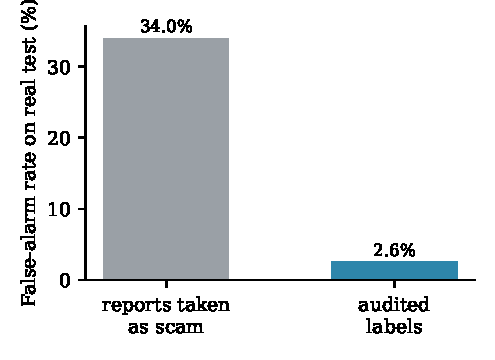
\includegraphics[width=0.55\linewidth]{figures/label_audit.pdf}
\caption{False-alarm rate with report labels and with audited labels}
\label{fig:audit}
\end{figure}
Training the same model with every reported message labelled as a scam gives 99.4\% recall but flags 34.0\% of genuine messages. With audited labels the false-alarm rate is 2.6\% at 97.6\% recall. The difference is highly significant (210 against 23 discordant messages, McNemar $p<10^{-30}$). This is the clearest result of the project: checking the labels mattered far more than choosing the algorithm.

\section{Effect of the split and of synthetic data}
With a random split of the real data, 793 test messages had a near-duplicate in training. The random split gave an F1 of 98.3\% and a 0.8\% false-alarm rate; the campaign-aware split gave 97.7\% and 1.4\%. The random split hides nearly half of the false alarms.

\begin{table}[H]
\centering
\caption{Effect of the training data (logistic regression, word + char, \%)}
\label{tab:train}
\begin{tabular}{|l|r|r|r|r|}
\hline
\textbf{Training data} & \textbf{Real F1} & \textbf{Real FAR} & \textbf{Challenge recall} & \textbf{Challenge F1} \\
\hline
Synthetic only & 87.4 & 31.1 & 86.4 & 90.3 \\
\hline
Real only & 97.7 & 1.4 & 35.6 & 51.2 \\
\hline
Real + synthetic & 98.1 & 2.6 & 82.2 & 90.2 \\
\hline
\end{tabular}
\end{table}
Synthetic messages alone do not resemble real Indian SMS closely enough. Real messages alone miss most of the newest scam types. Together they keep real-data F1 at 98.1\% and raise challenge F1 from 51.2\% to 90.2\%, at the cost of a slightly higher false-alarm rate.

\section{Value of the intent rules}
\label{sec:fusionexp}
\begin{table}[H]
\centering
\caption{Classifier alone and with fusion (\%)}
\label{tab:fusion}
\begin{tabular}{|l|r|r|r|}
\hline
\textbf{System} & \textbf{Real F1} & \textbf{Real false alarms} & \textbf{Challenge F1} \\
\hline
Classifier only & 98.1 & 2.6 & 90.2 \\
\hline
Hand-weighted rules (deployed) & 97.7 & 3.2 & 95.6 \\
\hline
Learned fusion weights & 98.3 & 2.3 & 91.2 \\
\hline
\end{tabular}
\end{table}
On real messages from unseen campaigns, the hand-weighted rules do not improve accuracy and add a few false alarms. On the team's own challenge messages they look much better. Learned fusion weights are significantly better than the hand-set ones on real data ($p=0.002$). We keep the rules in the application because they produce the phrase-level explanations and cover 2025--26 scam types that the real training data barely contains, but we do not claim that they improve accuracy.

\section{Operating point and errors}
\begin{figure}[H]
\centering
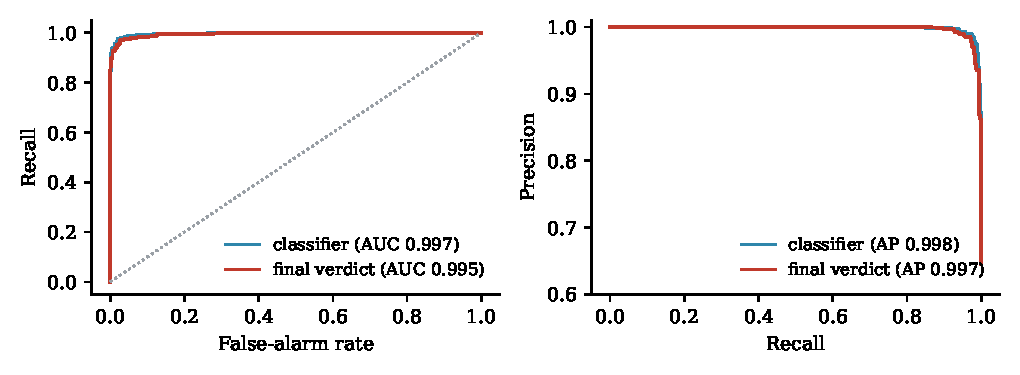
\includegraphics[width=0.95\linewidth]{figures/roc_pr.pdf}
\caption{ROC and precision-recall curves on the real test set}
\label{fig:rocpr}
\end{figure}
\begin{figure}[H]
\centering
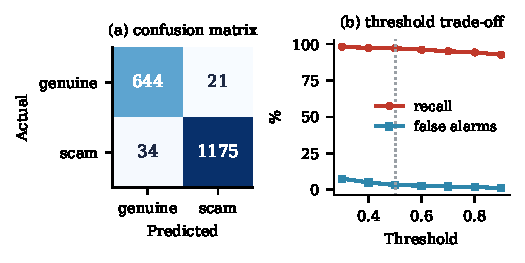
\includegraphics[width=0.7\linewidth]{figures/confusion.pdf}
\caption{(a) Confusion matrix of the deployed system; (b) recall and false-alarm rate by threshold}
\label{fig:conf}
\end{figure}
The deployed score has a ROC-AUC of 0.995. At the default threshold it misses 34 of 1,209 scams and flags 21 of 665 genuine messages. Fifteen of these 21 are reported-but-genuine bank messages that ask the user to click a link to finish a KYC or card application, which are hard even for people. A threshold of 0.9 would lower false alarms to 0.8\% at 92.5\% recall. Recall is 97.7\% on banking scams (895 of 916) and 92.3\% on government-themed scams (24 of 26). Obfuscating keywords in 837 test scams lowered recall from 99.4\% to 98.9\% with word features and to 99.3\% with word and character features.

The model and vectorizer take 1.6~MB on disk, training takes 2.7 seconds, and scoring one message takes about 2~ms (4~ms with the rules).

\section{Application snapshots}
Selected screens of the deployed application are shown in Appendix A.

% ======================================================================
\chapter{Conclusion and Future Work}

\section{Conclusion}
ScamGuard detects scam and fraud SMS for Indian users and explains each verdict. The main lesson of the project is about data. A model trained on user reports taken at face value flagged 34.0\% of genuine messages. The same model trained on the audited ScamGuard-IN-2026 corpus flags 2.6\% while catching 97.6\% of scams, and the deployed system reaches 97.1\% accuracy on real messages from unseen campaigns. Splitting the data by scam campaign gave a more honest estimate of false alarms than a random split, and comparing rules on independent real data showed that rules mainly serve explanation.

The result is a deployed application that answers in milliseconds, explains every verdict at phrase level, supports Hindi, and offers tools for the situations around a scam message: a QR code, a UPI request, a suspicious file, a conversation that turned into a request for money.

\section{Future Work}
\begin{itemize}
\item Complete the team-contributed 2026 test set (R4) and repeat the evaluation on it, since it is the only real test of 2025--26 scam types.
\item Add a second annotator for the label audit and report agreement.
\item Extend to Kannada, Tamil, Telugu and other Indian languages.
\item Evaluate against adaptive attackers, including paraphrases generated by language models.
\item Compare with small transformer models under the same campaign-aware protocol, within the memory budget of a free server.
\item Use learned fusion weights in production once the 2026 test set confirms that they do not lose the coverage of the newest scam types.
\item Offer the detector as an Android share target so that users can check a message without copying it.
\end{itemize}

\clearpage
% ----- References -----
\renewcommand{\bibname}{REFERENCES}
\begin{thebibliography}{99}
\addcontentsline{toc}{chapter}{REFERENCES}
\bibitem{agarwal2025fishing} S. Agarwal, A. Papasavva, G. Suarez-Tangil, and M. Vasek, ``Fishing for smishing: Understanding SMS phishing infrastructure and strategies by mining public user reports,'' in \textit{Proc. ACM Internet Measurement Conference (IMC '25)}, Madison, WI, USA, 2025, doi: 10.1145/3730567.3764431.
\bibitem{agarwal2026overview} S. Agarwal, G. Suarez-Tangil, and M. Vasek, ``An overview of 7726 user reports: Uncovering SMS scams and scammer strategies,'' in \textit{Proc. Network and Distributed System Security Symposium (NDSS)}, San Diego, CA, USA, 2026.
\bibitem{pritom2026sms} M. M. A. Pritom, S. M. Sanjari, M. Mia, A. M. Shibli, S. M. M. Hossain, M. Ismail, and S. Xu, ``Short message service (SMS) phishing attacks and defenses: A systematic review,'' arXiv:2604.11429, 2026.
\bibitem{almeida2011contributions} T. A. Almeida, J. M. G\'omez Hidalgo, and A. Yamakami, ``Contributions to the study of SMS spam filtering: New collection and results,'' in \textit{Proc. 11th ACM Symposium on Document Engineering}, Mountain View, CA, USA, 2011, pp. 259--262.
\bibitem{almeida2013towards} T. A. Almeida, J. M. G\'omez Hidalgo, and T. P. Silva, ``Towards SMS spam filtering: Results under a new dataset,'' \textit{International Journal of Information Security Science}, vol. 2, no. 1, pp. 1--18, 2013.
\bibitem{roy2020deep} P. K. Roy, J. P. Singh, and S. Banerjee, ``Deep learning to filter SMS spam,'' \textit{Future Generation Computer Systems}, vol. 102, pp. 524--533, 2020.
\bibitem{mishra2020smishing} S. Mishra and D. Soni, ``Smishing Detector: A security model to detect smishing through SMS content analysis and URL behavior analysis,'' \textit{Future Generation Computer Systems}, 2020.
\bibitem{sonowal2018smidca} G. Sonowal and K. S. Kuppusamy, ``SmiDCA: An anti-smishing model with machine learning approach,'' \textit{The Computer Journal}, vol. 61, no. 8, pp. 1143--1157, 2018, doi: 10.1093/comjnl/bxy039.
\bibitem{goel2024ml} D. Goel, H. Ahmad, A. K. Jain, and N. K. Goel, ``Machine learning driven smishing detection framework for mobile security,'' arXiv:2412.09641, 2024.
\bibitem{timko2024smishing} D. Timko and M. L. Rahman, ``Smishing Dataset I: Phishing SMS dataset from Smishtank.com,'' in \textit{Proc. 14th ACM Conference on Data and Application Security and Privacy (CODASPY '24)}, Porto, Portugal, 2024, doi: 10.1145/3626232.3653282.
\bibitem{ali2025moz} F. D. M. A. Ali, S. M. Saide, R. Sousa-Silva, and H. Lopes Cardoso, ``MOZ-Smishing: A benchmark dataset for detecting mobile money frauds,'' in \textit{Proc. 6th Workshop on African Natural Language Processing}, Vienna, Austria, 2025, pp. 158--166, doi: 10.18653/v1/2025.africanlp-1.23.
\bibitem{labonne2023spamt5} M. Labonne and S. Moran, ``Spam-T5: Benchmarking large language models for few-shot email spam detection,'' arXiv:2304.01238, 2023.
\bibitem{ahmadi2025llm} M. Ahmadi, M. Khajavi, A. Varmaghani, A. Ala, K. Danesh, and D. Javaheri, ``Leveraging large language models for cybersecurity: Enhancing SMS spam detection with robust and context-aware text classification,'' arXiv:2502.11014, 2025.
\bibitem{northcutt2021confident} C. Northcutt, L. Jiang, and I. Chuang, ``Confident learning: Estimating uncertainty in dataset labels,'' \textit{Journal of Artificial Intelligence Research}, vol. 70, pp. 1373--1411, 2021, doi: 10.1613/jair.1.12125.
\bibitem{lee2022dedup} K. Lee, D. Ippolito, A. Nystrom, C. Zhang, D. Eck, C. Callison-Burch, and N. Carlini, ``Deduplicating training data makes language models better,'' in \textit{Proc. 60th Annual Meeting of the ACL}, Dublin, Ireland, 2022, pp. 8424--8445, doi: 10.18653/v1/2022.acl-long.577.
\bibitem{kapoor2023leakage} S. Kapoor and A. Narayanan, ``Leakage and the reproducibility crisis in machine-learning-based science,'' \textit{Patterns}, 2023, doi: 10.1016/j.patter.2023.100804.
\bibitem{broder1997resemblance} A. Z. Broder, ``On the resemblance and containment of documents,'' in \textit{Proc. Compression and Complexity of SEQUENCES 1997}, Positano, Italy, 1997, doi: 10.1109/SEQUEN.1997.666900.
\bibitem{salton1988term} G. Salton and C. Buckley, ``Term-weighting approaches in automatic text retrieval,'' \textit{Information Processing \& Management}, vol. 24, no. 5, pp. 513--523, 1988, doi: 10.1016/0306-4573(88)90021-0.
\bibitem{pedregosa2011scikit} F. Pedregosa \textit{et al.}, ``Scikit-learn: Machine learning in Python,'' \textit{Journal of Machine Learning Research}, vol. 12, pp. 2825--2830, 2011.
\end{thebibliography}
\clearpage

% ----- Appendices -----
\appendix
\renewcommand{\thefigure}{A.\arabic{figure}}
\renewcommand{\thetable}{E.\arabic{table}}
\setcounter{figure}{0}\setcounter{table}{0}
\renewcommand{\thechapter}{\Alph{chapter}}
\renewcommand{\thesection}{\Roman{section}}
\section*{Appendix A: Snapshots}
\addcontentsline{toc}{section}{Appendix A: Snapshots}
\begin{figure}[H]\centering\fbox{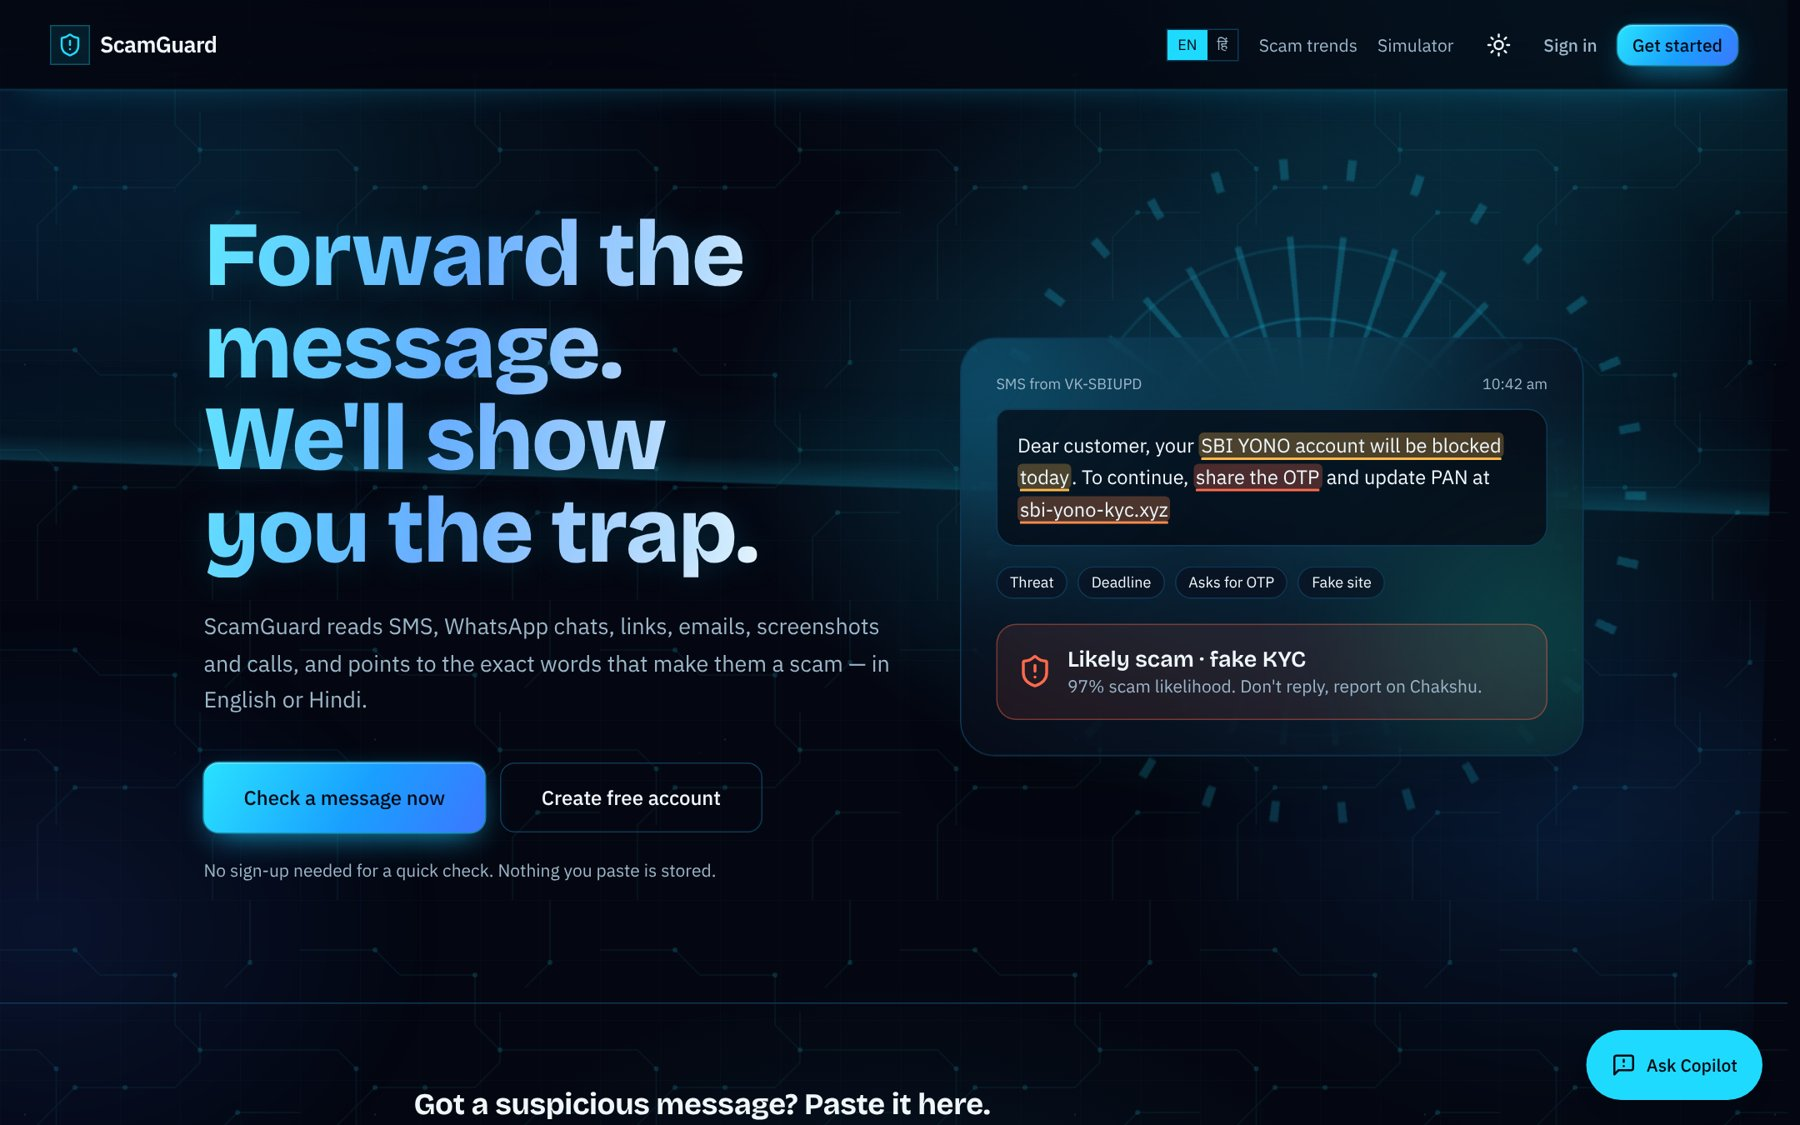
\includegraphics[width=0.82\linewidth]{shots/01_landing.jpg}}\caption{Home page with the quick check}\end{figure}
\begin{figure}[H]\centering\fbox{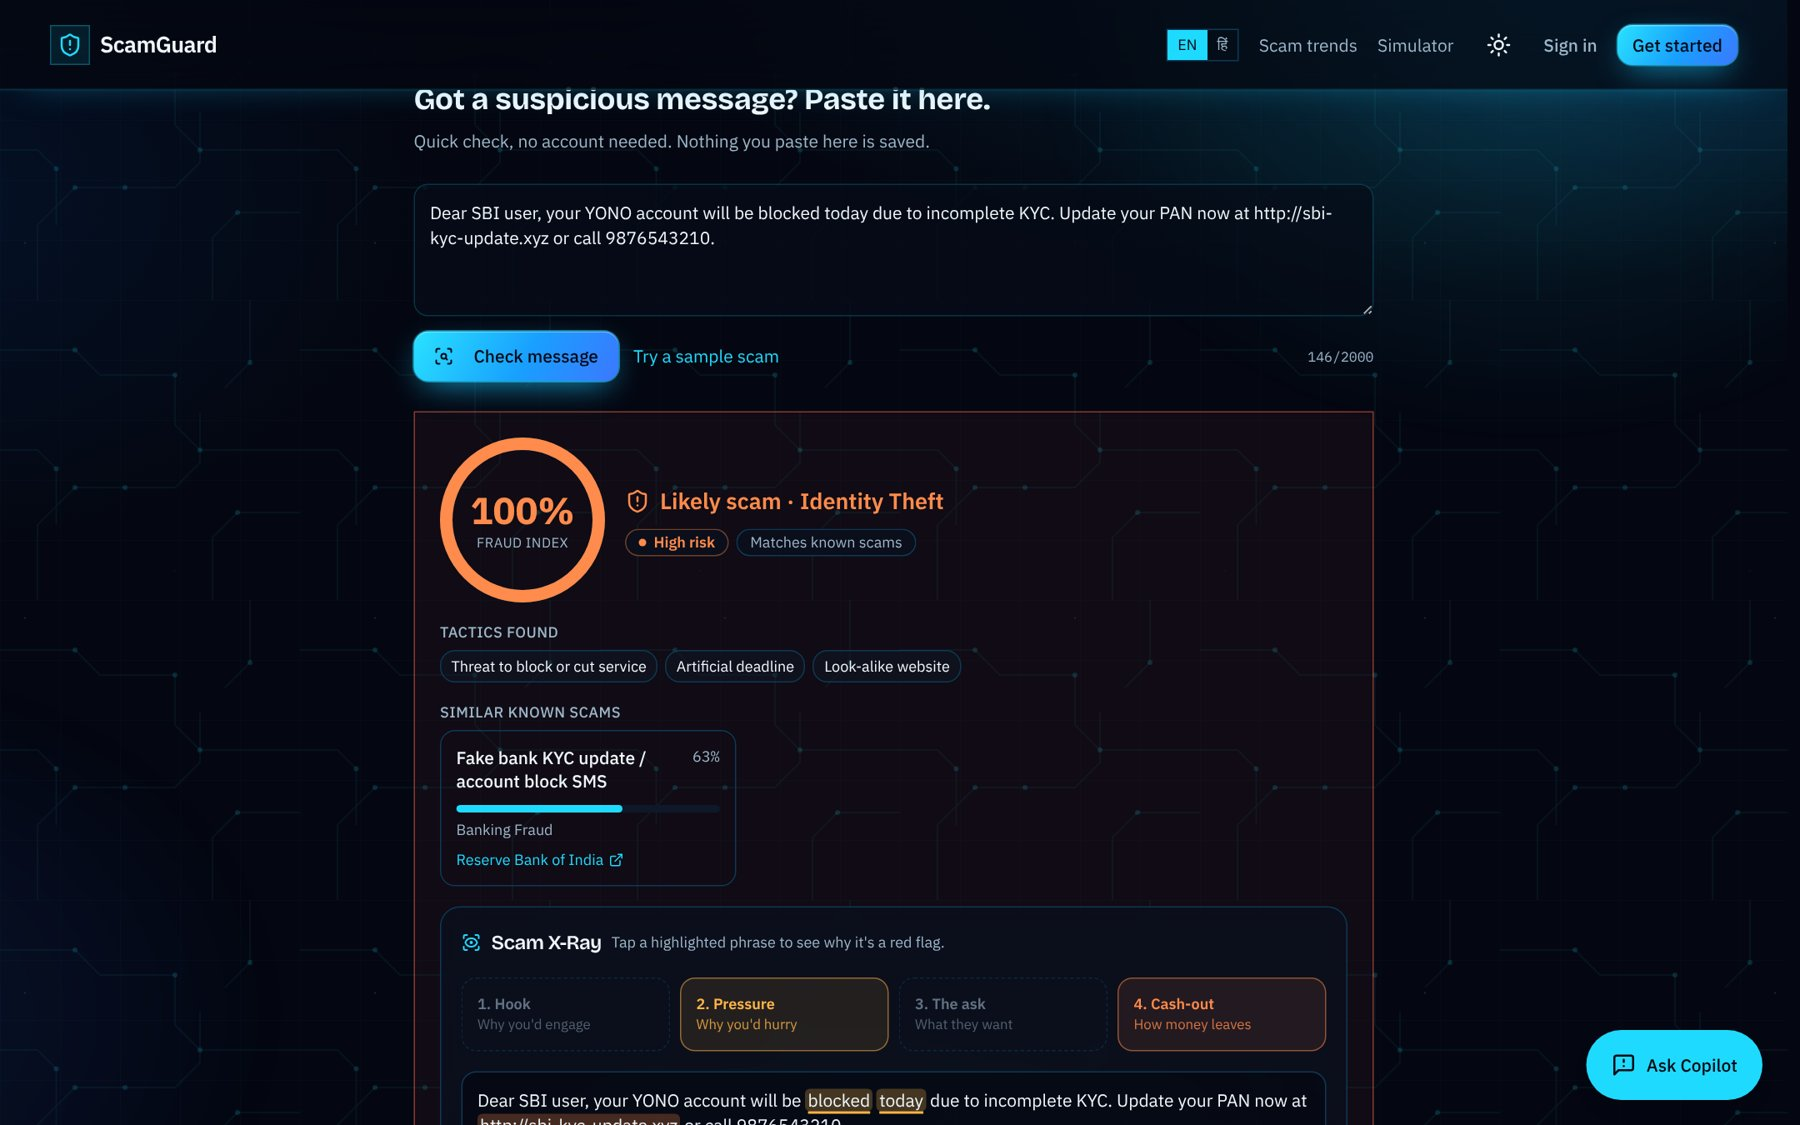
\includegraphics[width=0.82\linewidth]{shots/02_quick_scam.jpg}}\caption{Quick check of a fake KYC message: verdict, matched tactics, known pattern and Scam X-Ray}\end{figure}
\begin{figure}[H]\centering\fbox{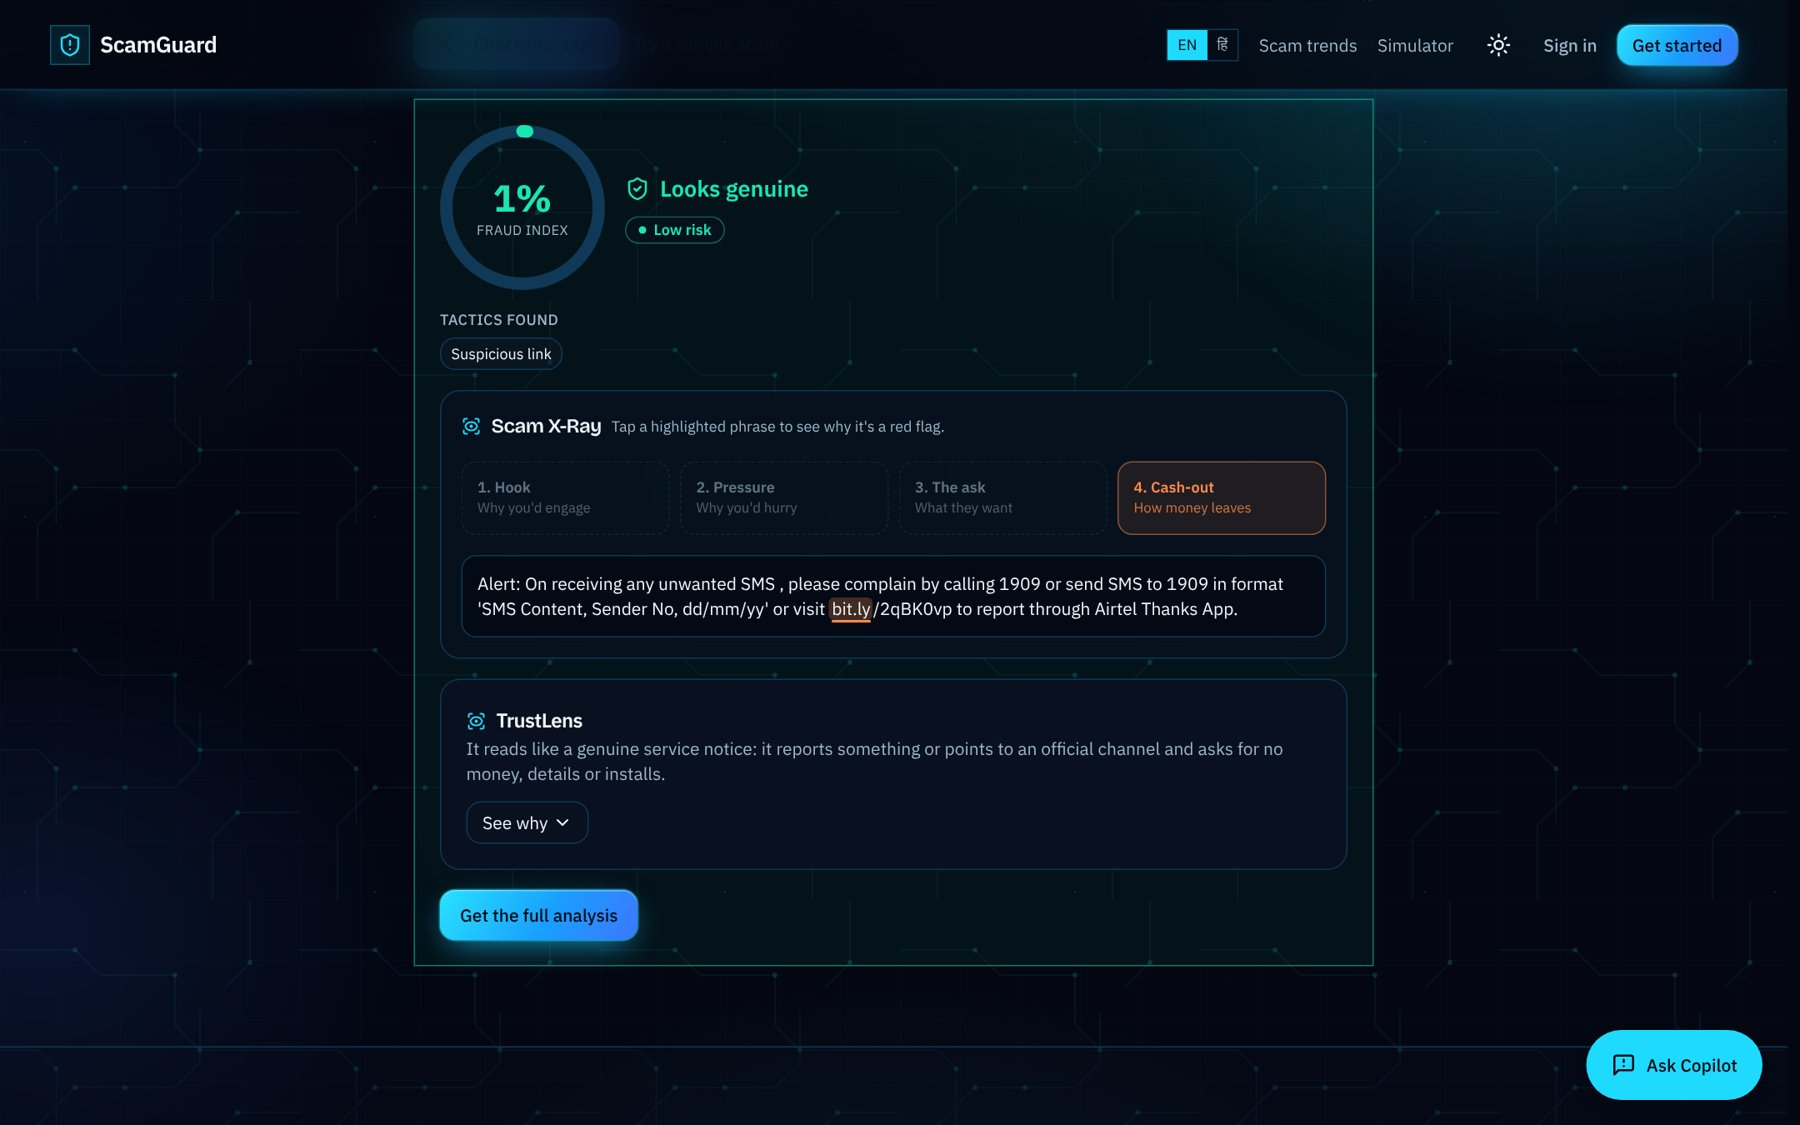
\includegraphics[width=0.82\linewidth]{shots/03_quick_genuine.jpg}}\caption[Quick check of a genuine operator notice]{Quick check of a genuine operator notice about the 1909 helpline: ``Looks genuine'' with the TrustLens reason}\end{figure}
\begin{figure}[H]\centering\fbox{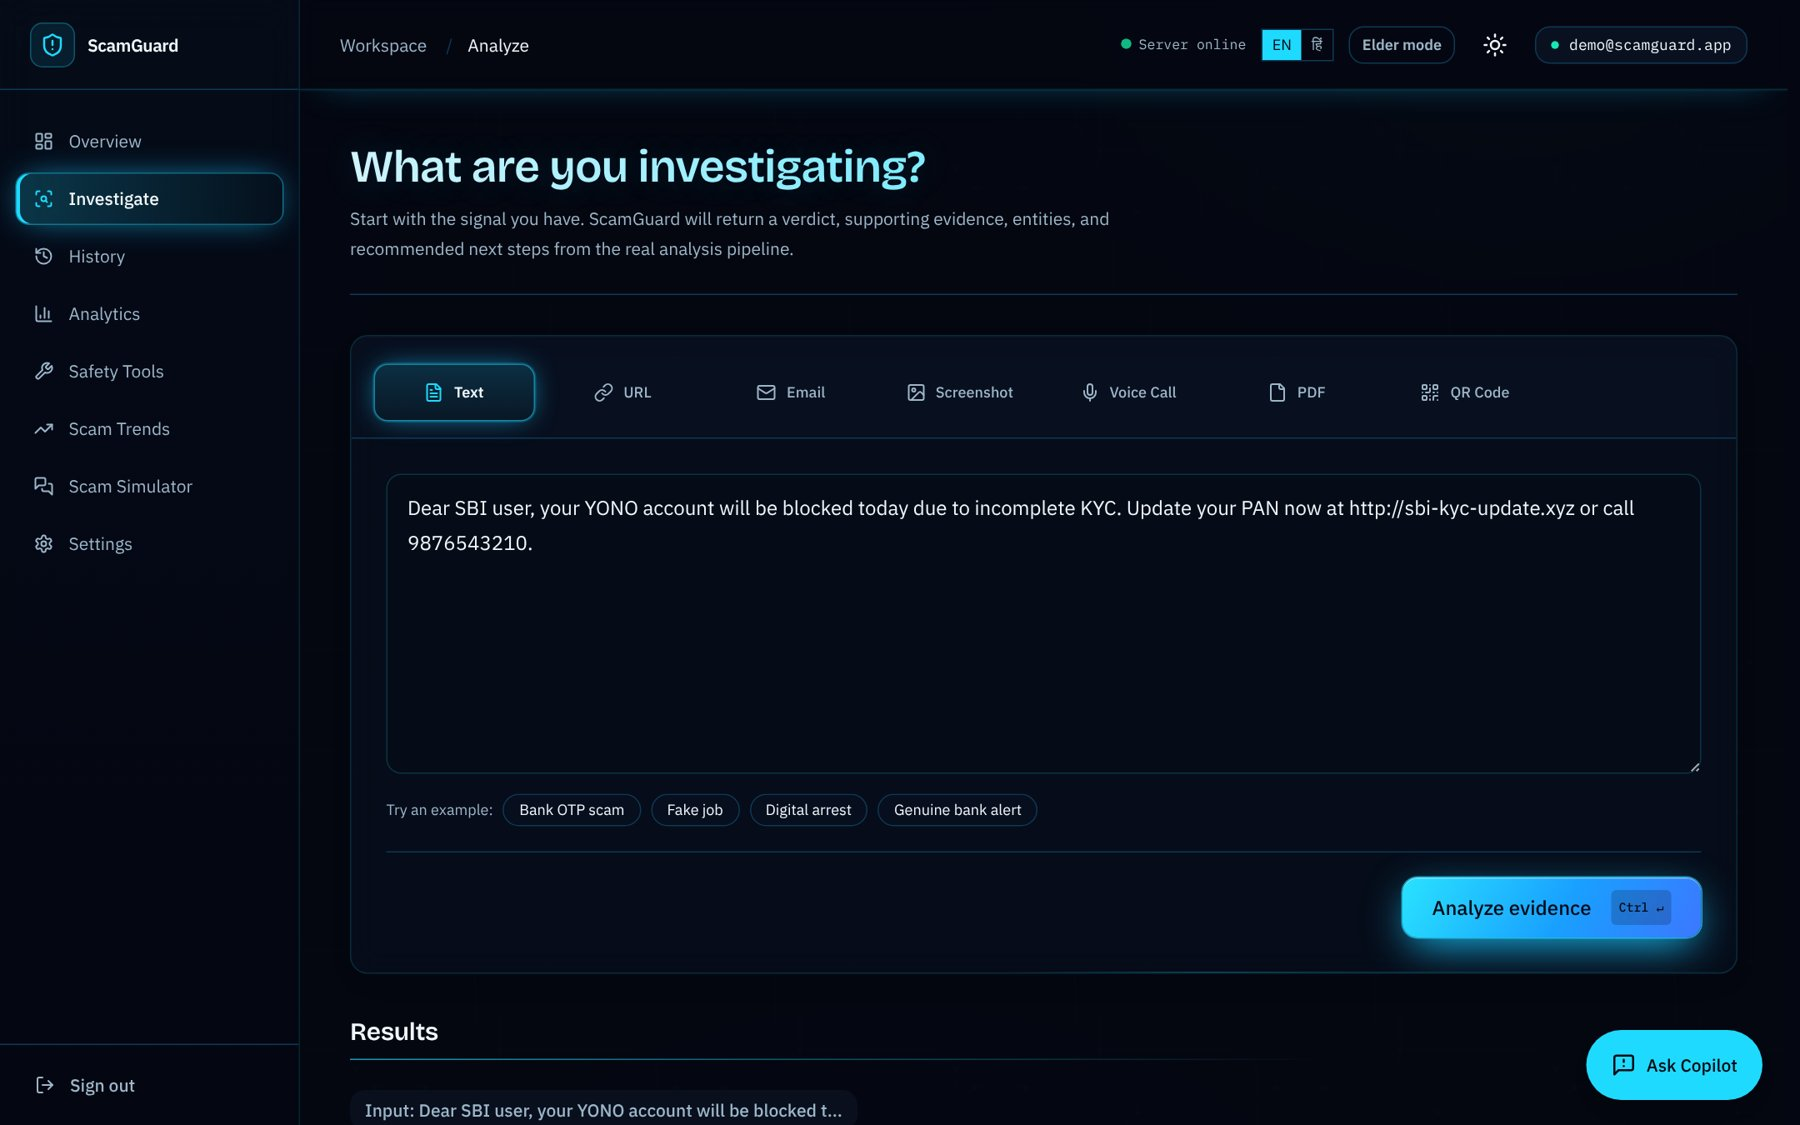
\includegraphics[width=0.82\linewidth]{shots/05_analyze_result.jpg}}\caption{Full analysis of a scam message for a signed-in user}\end{figure}
\begin{figure}[H]\centering\fbox{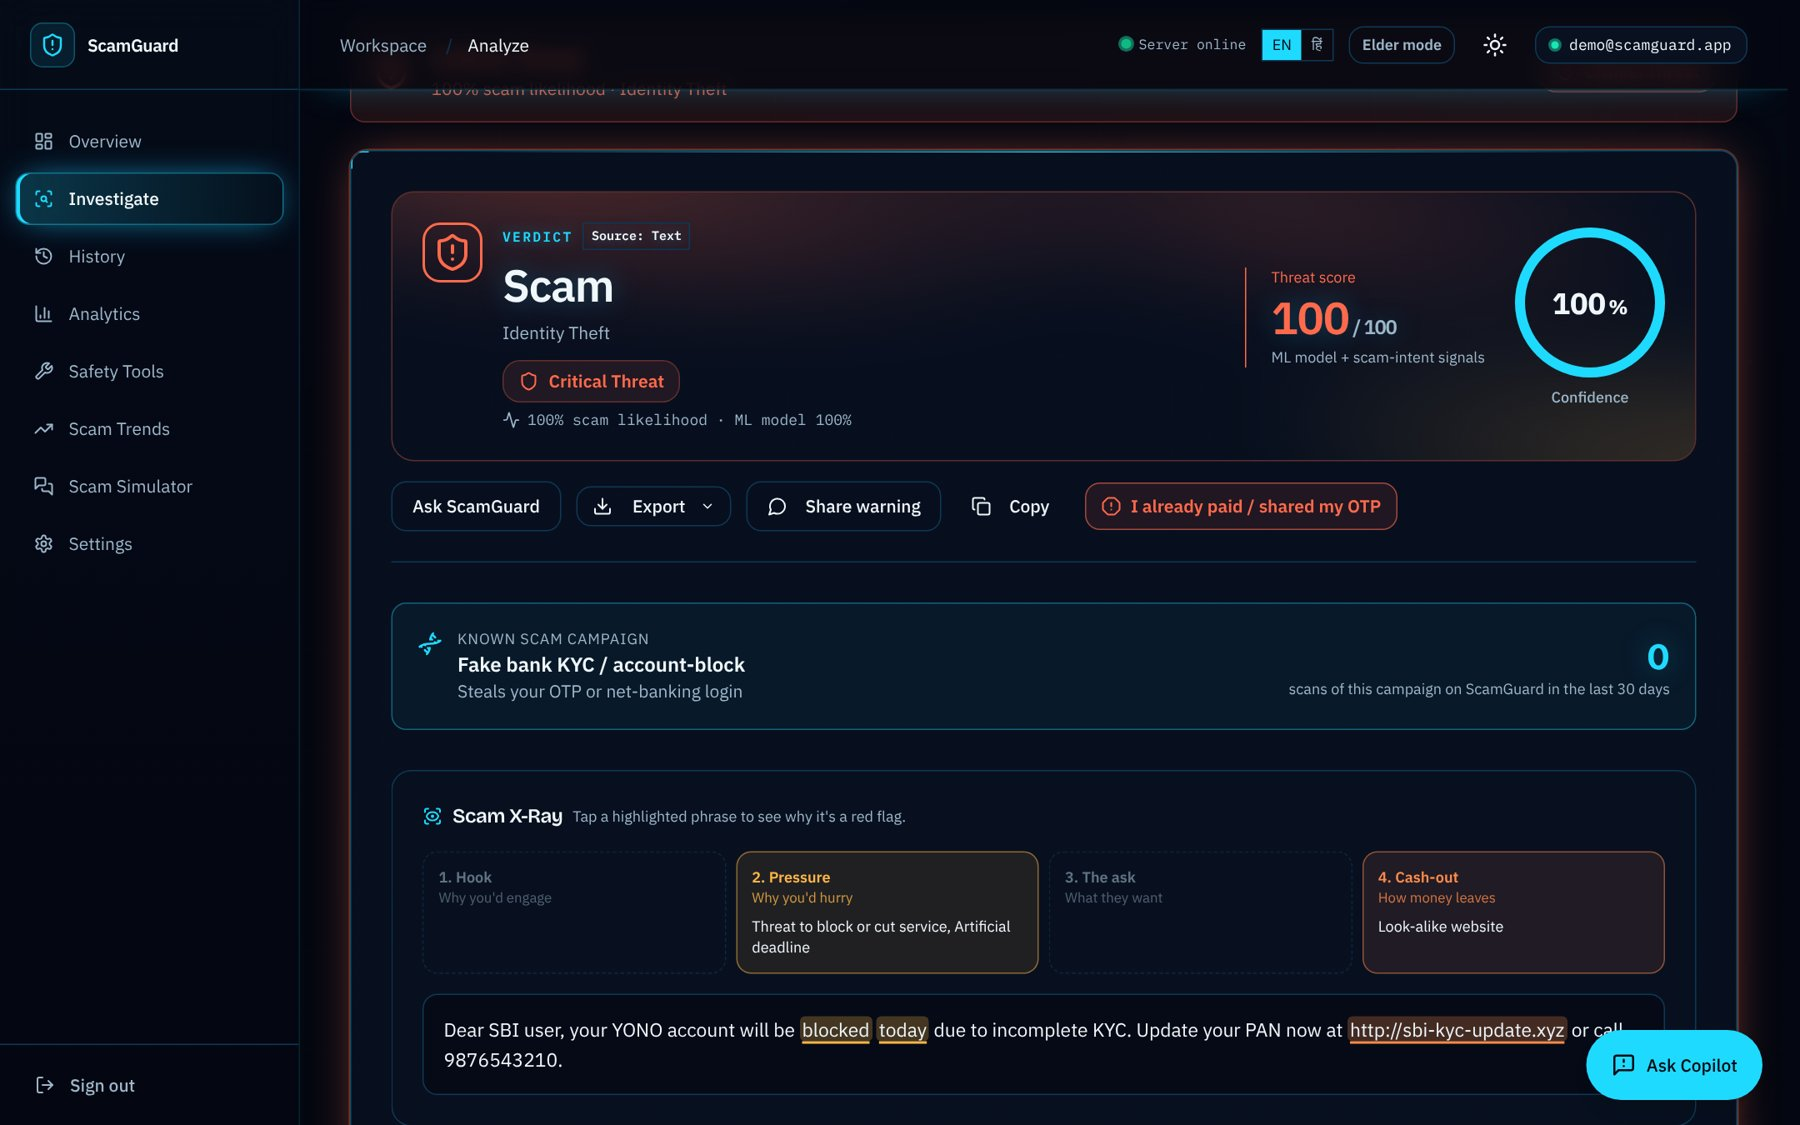
\includegraphics[width=0.82\linewidth]{shots/06_analyze_xray.jpg}}\caption{Scam X-Ray: each risky phrase placed in the hook, pressure, request and cash-out stages}\end{figure}
\begin{figure}[H]\centering\fbox{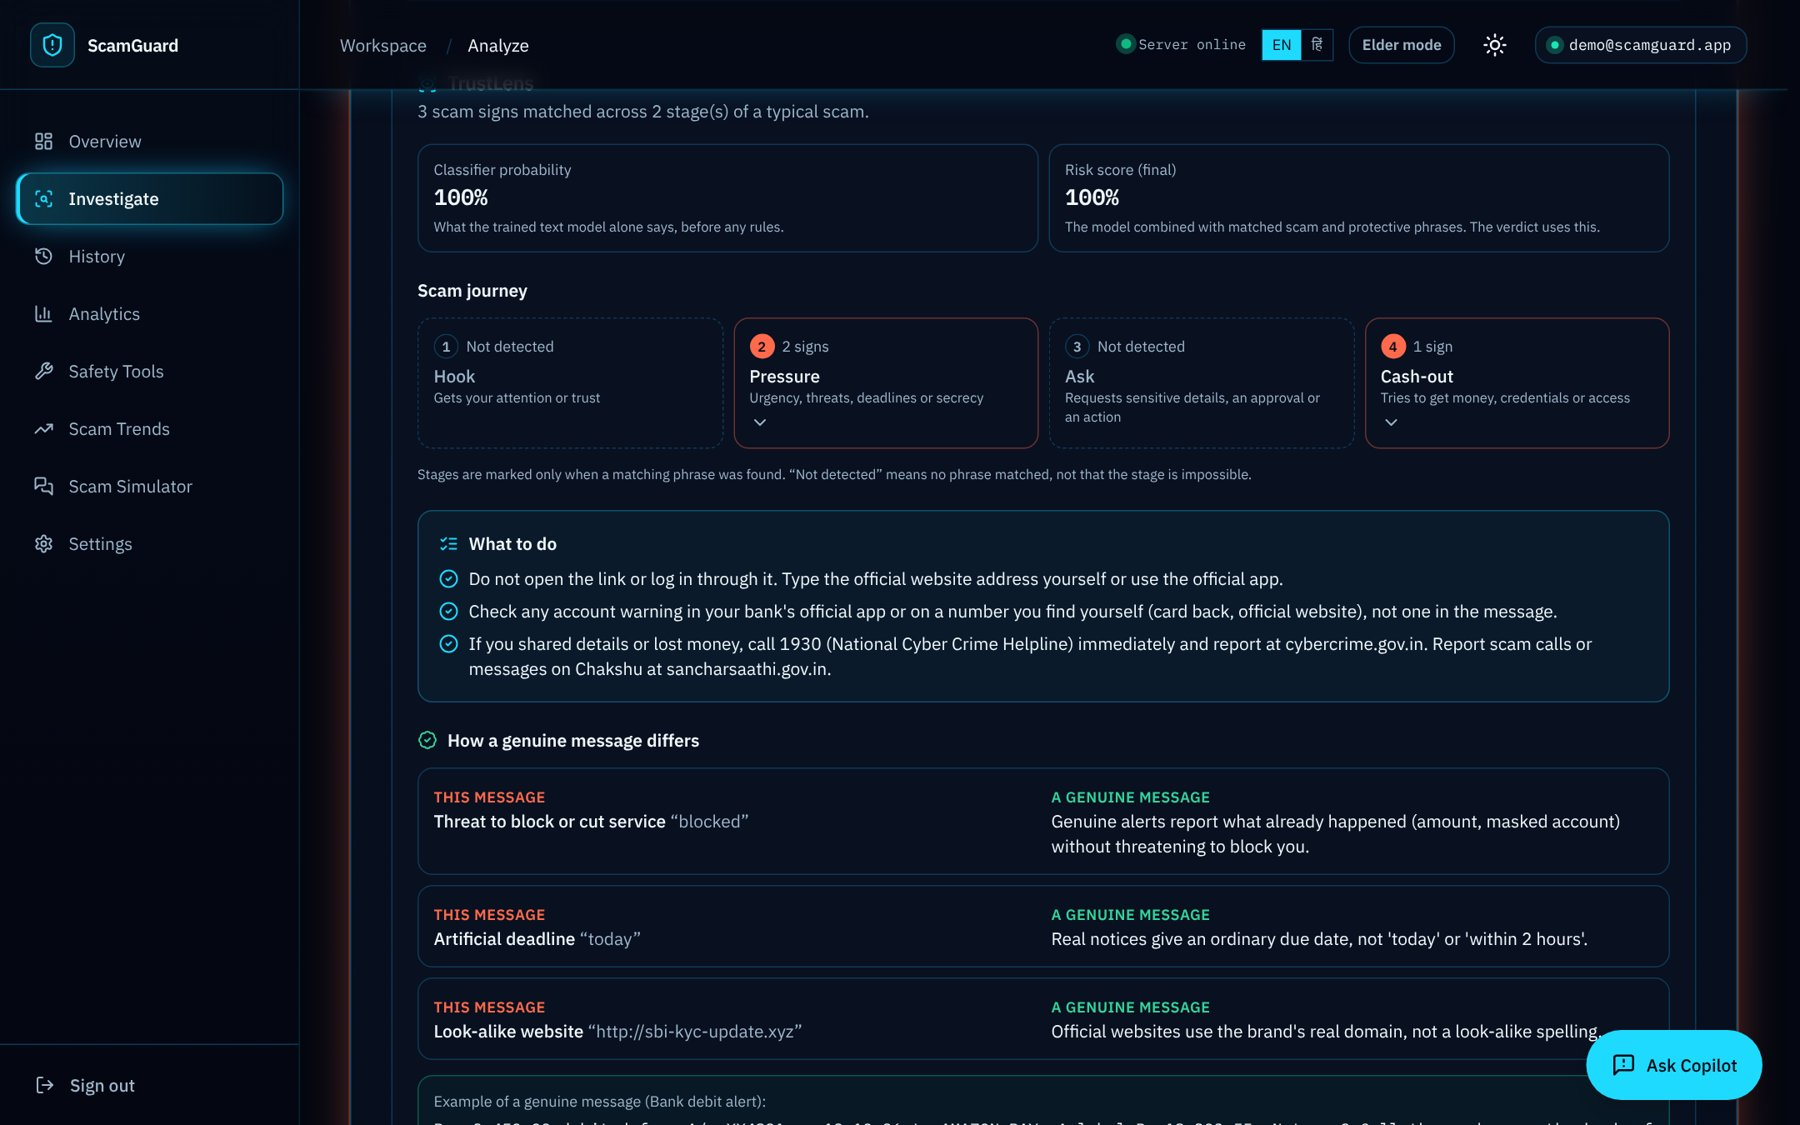
\includegraphics[width=0.82\linewidth]{shots/07_analyze_trustlens.jpg}}\caption{TrustLens: scam journey, recommended actions and how a genuine message differs}\end{figure}
\begin{figure}[H]\centering\fbox{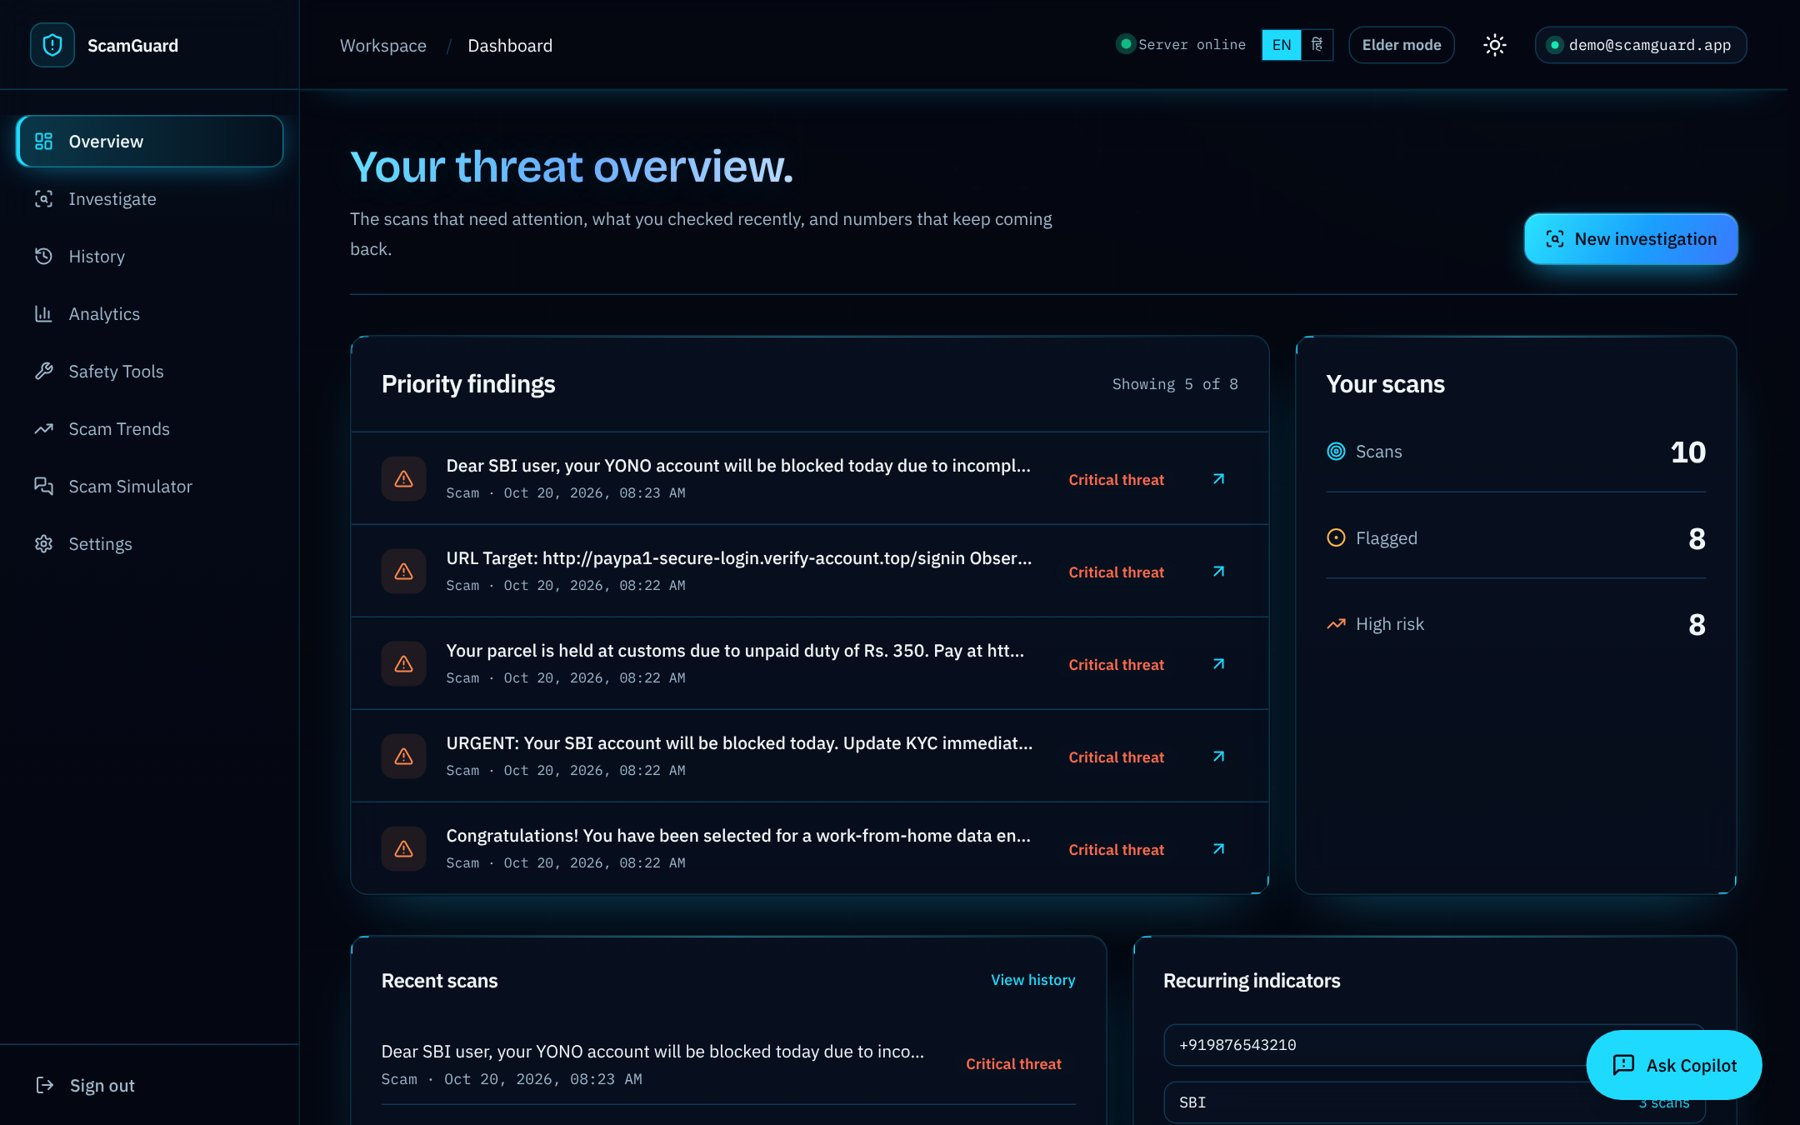
\includegraphics[width=0.82\linewidth]{shots/08_dashboard.jpg}}\caption{Dashboard with priority findings and recent scans}\end{figure}
\begin{figure}[H]\centering\fbox{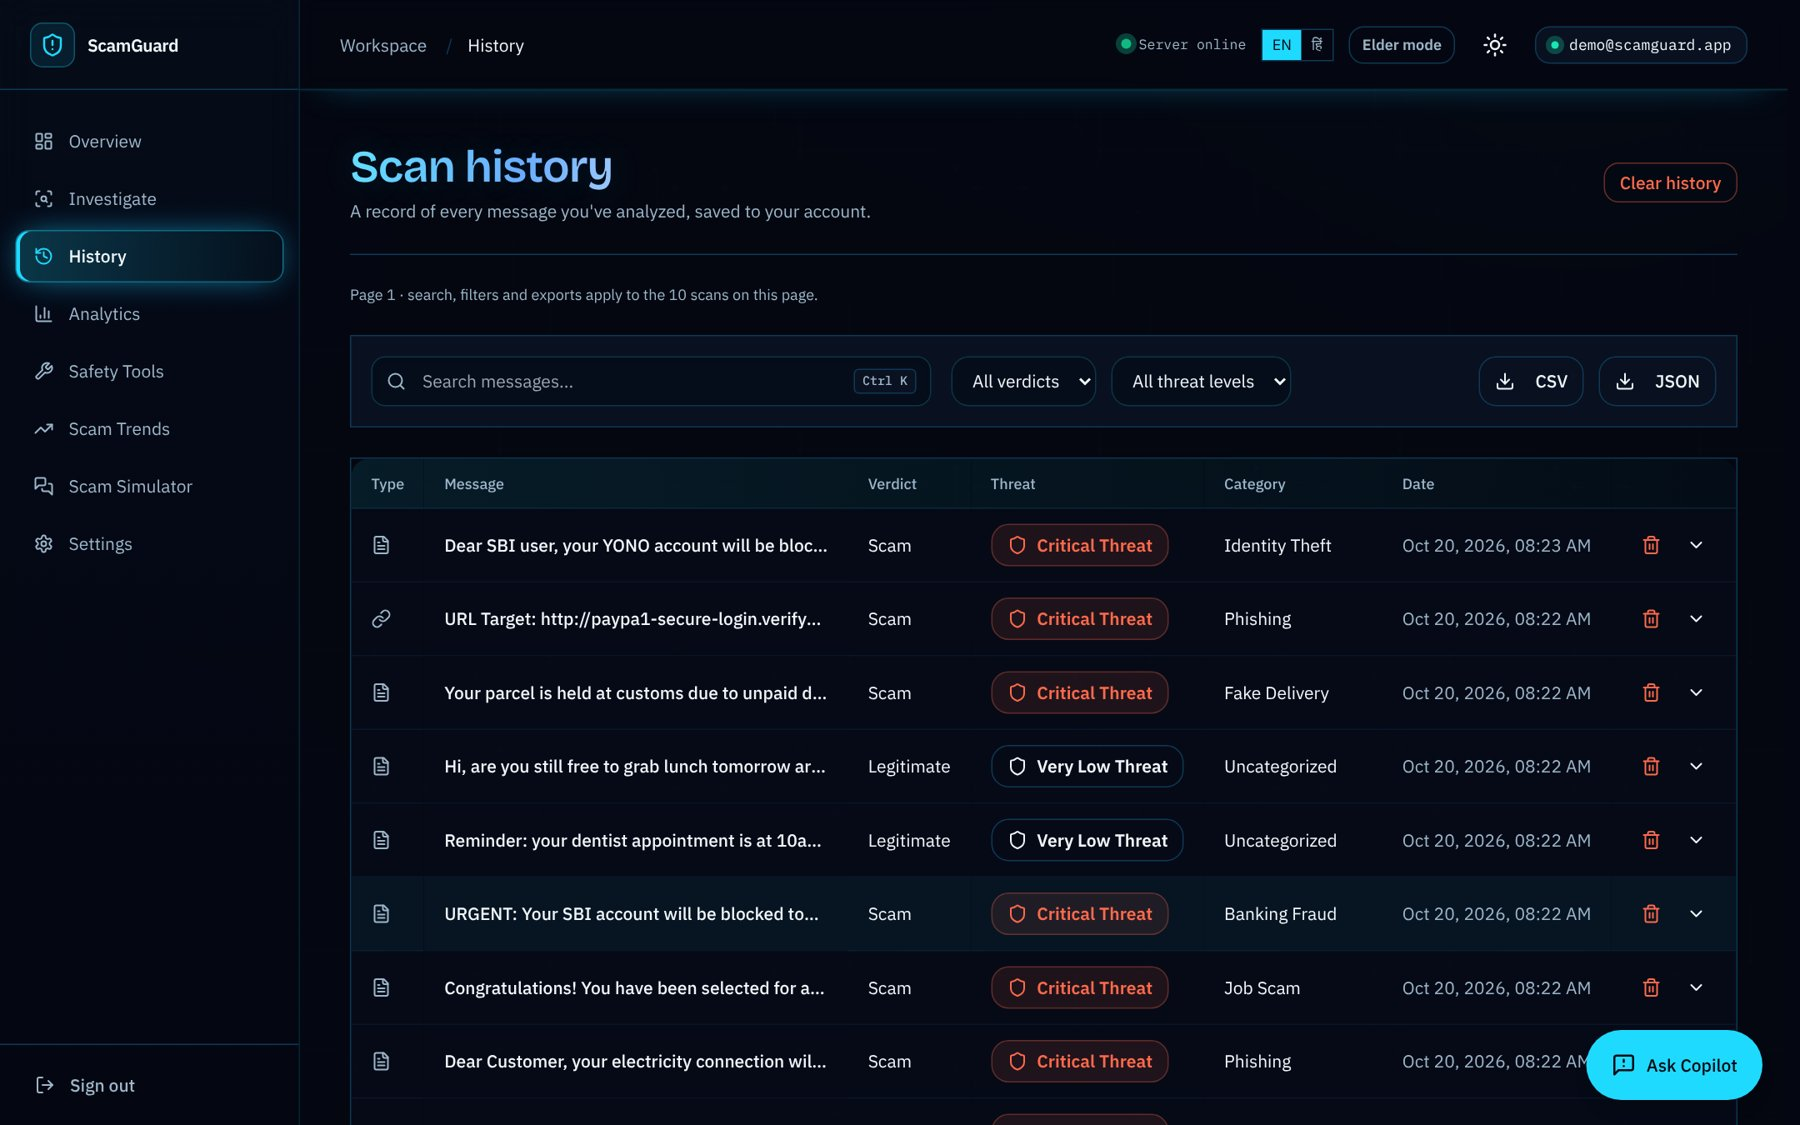
\includegraphics[width=0.82\linewidth]{shots/09_history.jpg}}\caption{Scan history with search, filters and export}\end{figure}
\begin{figure}[H]\centering\fbox{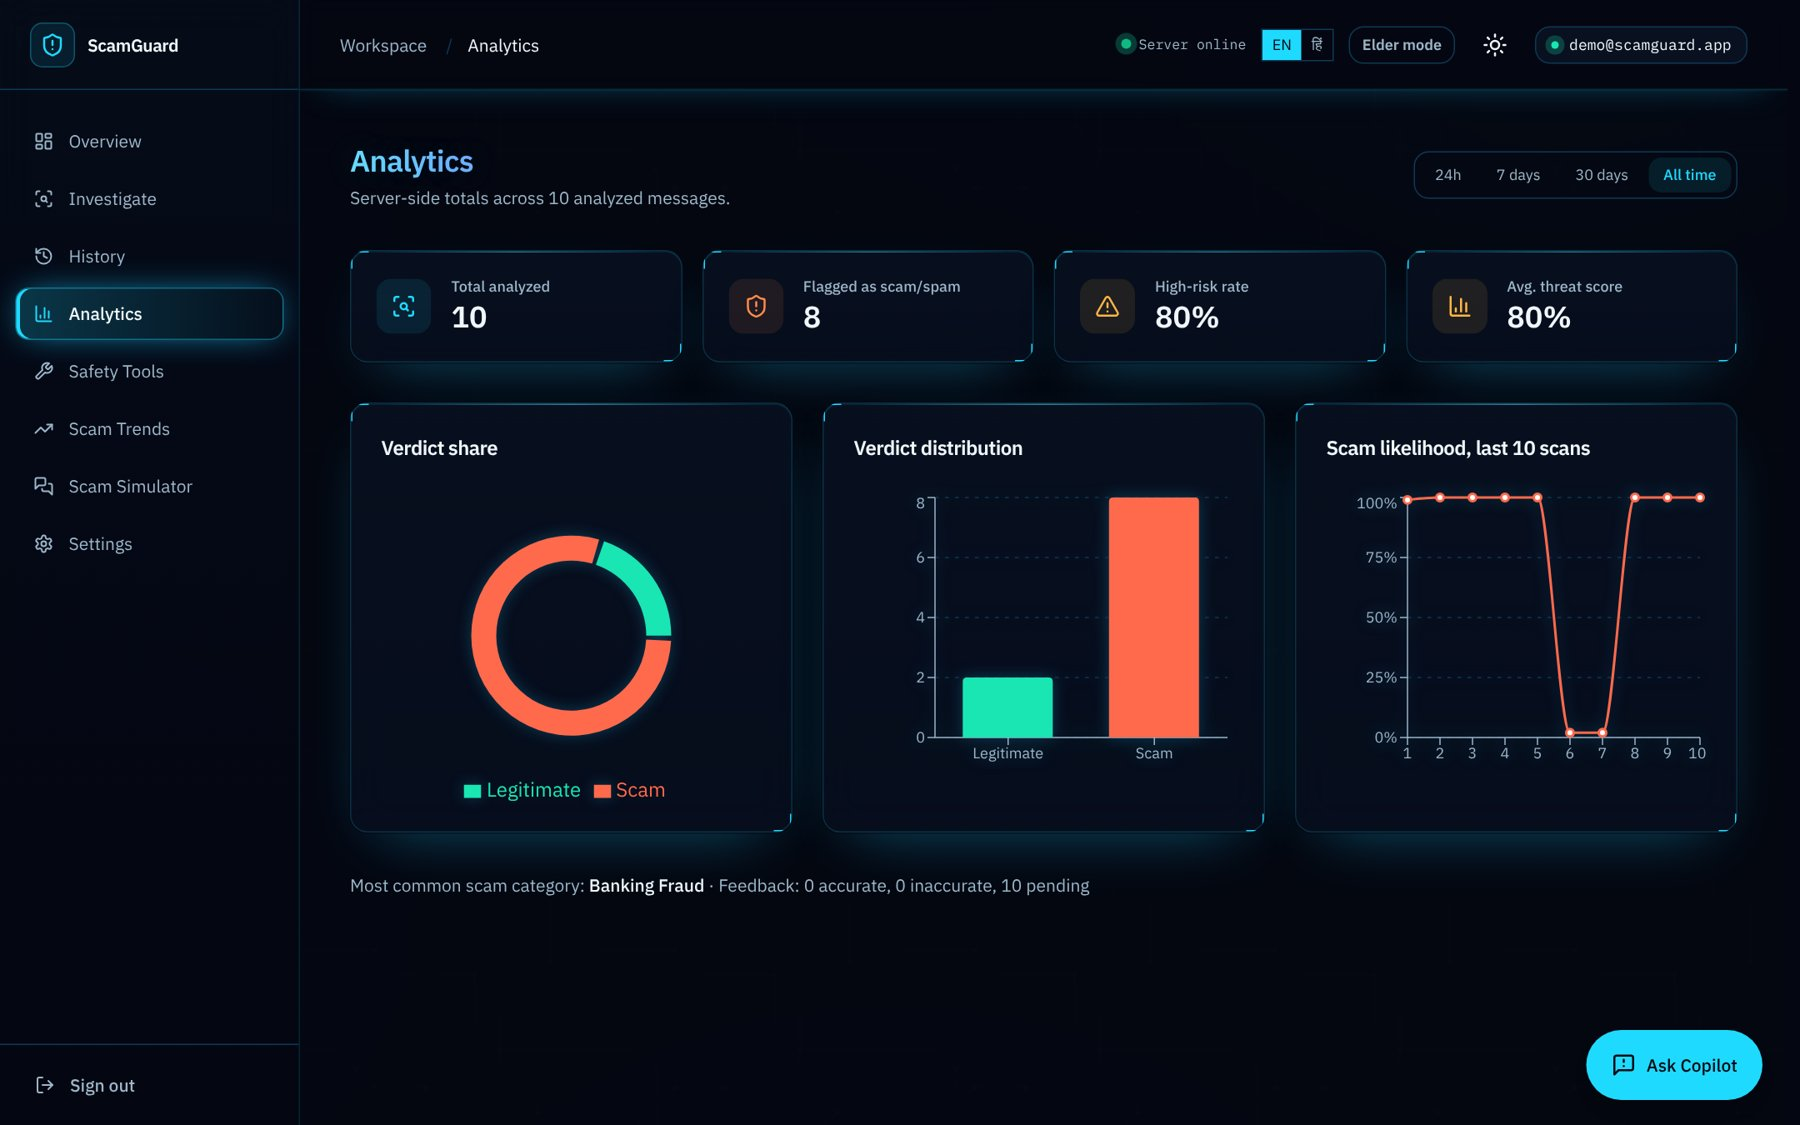
\includegraphics[width=0.82\linewidth]{shots/10_analytics.jpg}}\caption{Analytics: verdict share, distribution and score trend}\end{figure}
\begin{figure}[H]\centering\fbox{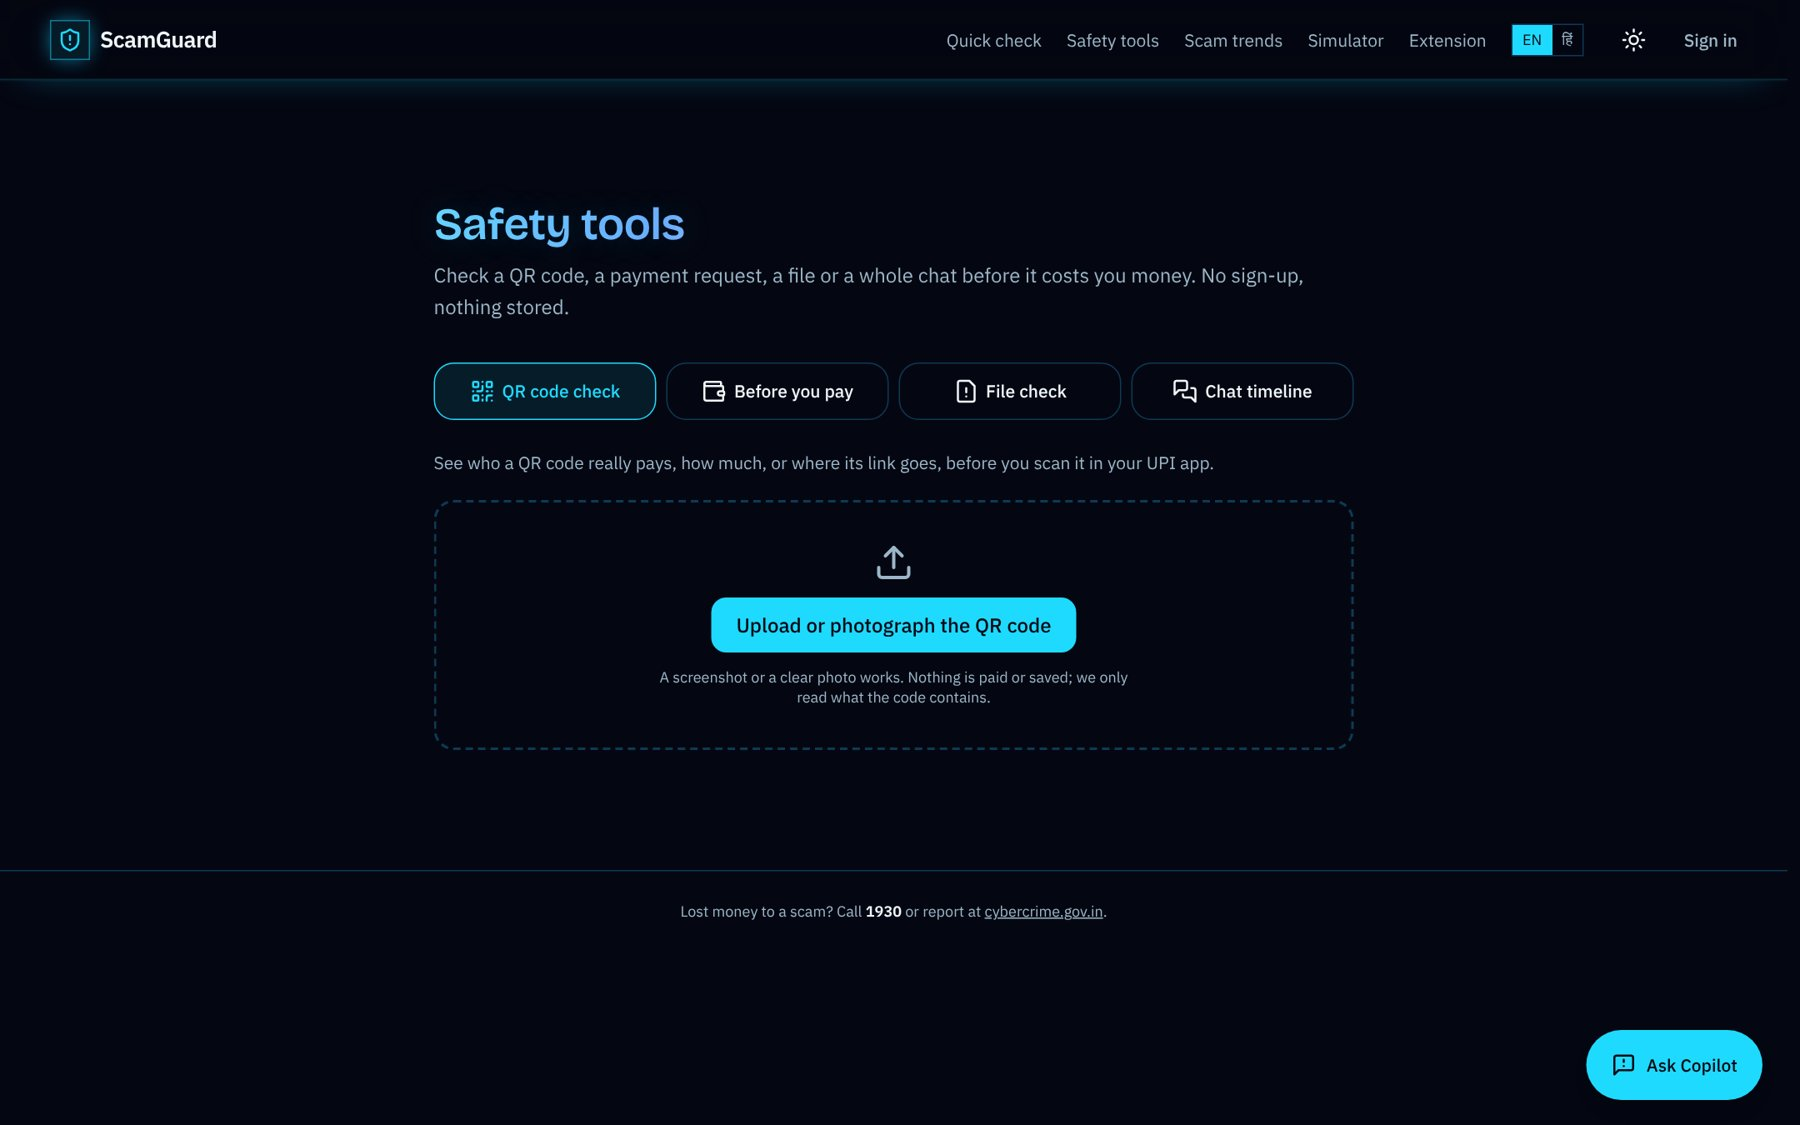
\includegraphics[width=0.82\linewidth]{shots/11_tools.jpg}}\caption{Safety tools: QR code check, before-you-pay, file check and chat timeline}\end{figure}
\begin{figure}[H]\centering\fbox{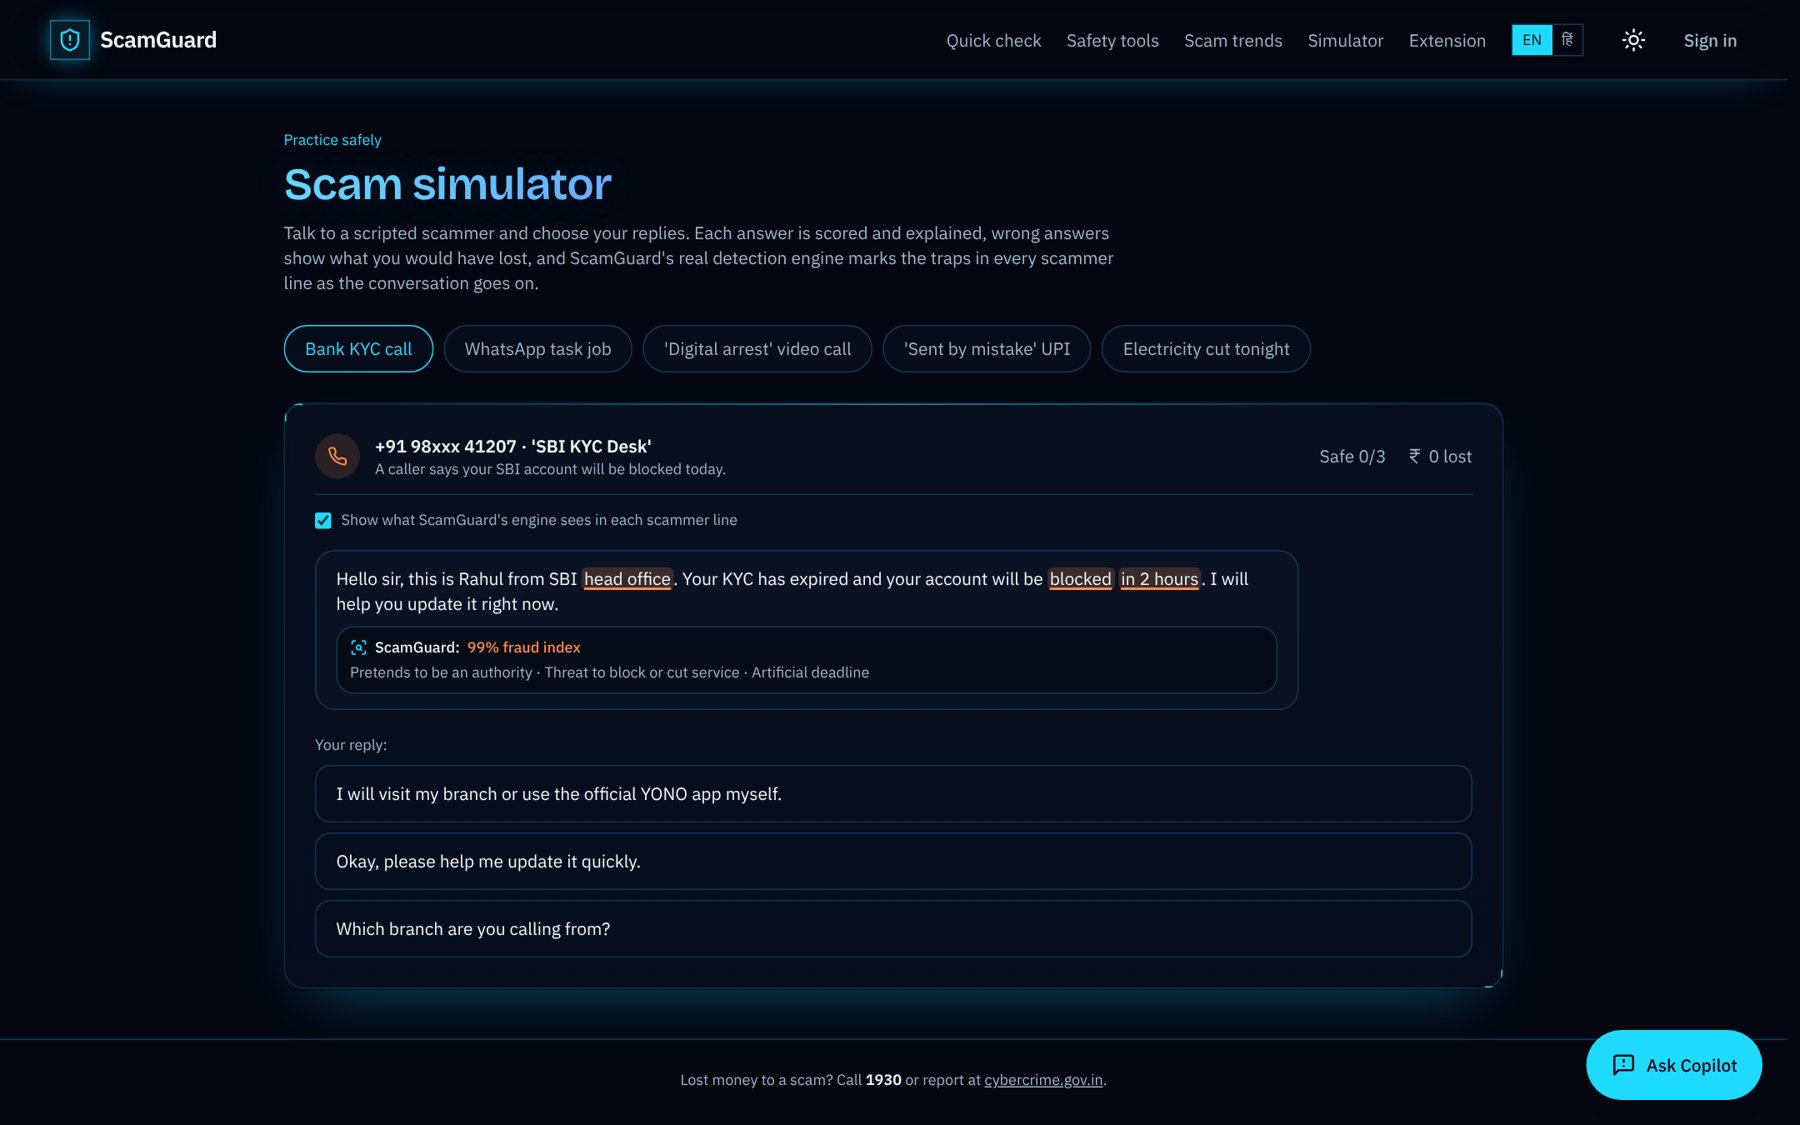
\includegraphics[width=0.82\linewidth]{shots/12_simulator.jpg}}\caption{Scam simulator for practice}\end{figure}
\clearpage
\section*{Appendix B: Details of list of publications related to this project}
\addcontentsline{toc}{section}{Appendix B: Details of list of publications related to this project}
\large{Author Names: } Kayarvizhy N, Priyam Thakur, Bhavya Goyal, Samir Chaudhary, Sana Subodh \\
\large{Paper Title: } ScamGuard: AI-Based Online Scam and Fraud Detection System \\
\large {Name of the Conference or Journal:} To be decided (manuscript prepared in IEEE conference format) \\
\large {Place of the conference:} -- \\
\large {Date of Conference:} --
\clearpage
\section*{Appendix C: Details of Patent}
\addcontentsline{toc}{section}{Appendix C: Details of Patent}
No patent has been filed for this project.
\clearpage
\section*{Appendix D: Details of Funding}
\addcontentsline{toc}{section}{Appendix D: Details of Funding}
The project received no external funding. It was built with free cloud tiers and open-source software.
\clearpage
\section*{Appendix E: POs and PSOs Mapped}
\addcontentsline{toc}{section}{Appendix E: POs and PSOs Mapped}
{\small
\renewcommand{\arraystretch}{1.2}
\setlength{\tabcolsep}{6pt}
\begin{longtable}{|L{3.6cm}|c|L{7.2cm}|}
\caption{Programme Outcomes Mapping with Project}\\
\hline
\textbf{PROGRAMME OUTCOMES} & \textbf{Level (1/2/3)} & \textbf{Justification if addressed} \\
\hline
\endfirsthead
\hline
\textbf{PROGRAMME OUTCOMES} & \textbf{Level (1/2/3)} & \textbf{Justification if addressed} \\
\hline
\endhead
PO1 & 3 & Applies machine learning, NLP and statistics to classify scam messages and to evaluate the classifier. \\
\hline
PO2 & 3 & Analyses why existing filters fail on Indian SMS and traces the failure to dataset labels and evaluation leakage. \\
\hline
PO3 & 3 & Designs a dataset, a detector and a web application that meet accuracy, latency and explanation requirements. \\
\hline
PO4 & 3 & Conducts controlled experiments with bootstrap intervals and significance tests on a campaign-held-out test set. \\
\hline
PO5 & 3 & Uses scikit-learn, FastAPI, Next.js, MinHash, GitHub Actions and cloud deployment. \\
\hline
PO6 & 3 & Protects users from financial fraud and points them to official reporting channels. \\
\hline
PO7 & 1 & Runs on free, low-power infrastructure; the detector needs no GPU. \\
\hline
PO8 & 3 & Masks personal data, respects dataset licences and reports limitations honestly. \\
\hline
PO9 & 3 & Built by a team of four with shared responsibility for data, model, back end and front end. \\
\hline
PO10 & 3 & Communicates results through a report, a research paper, a datasheet and an explanatory user interface. \\
\hline
PO11 & 2 & Plans the work in phases and keeps the deployment within free-tier budgets. \\
\hline
PO12 & 2 & Designs the dataset build so that new scam types and the 2026 test set can be added and re-evaluated. \\
\hline
\end{longtable}}


{\small
\renewcommand{\arraystretch}{1.2}
\setlength{\tabcolsep}{6pt}
\begin{longtable}{|L{3.6cm}|c|L{7.2cm}|}
\caption{Programme Specific Outcomes Mapping with Project}\\
\hline
\textbf{PROGRAMME SPECIFIC OUTCOMES} & \textbf{Level (1/2/3)} & \textbf{Justification if addressed} \\
\hline
\endfirsthead
\hline
\textbf{PROGRAMME SPECIFIC OUTCOMES} & \textbf{Level (1/2/3)} & \textbf{Justification if addressed} \\
\hline
\endhead
PSO1 & 2 & Uses web APIs, cloud hosting, rate limiting and secure token-based communication. \\
\hline
PSO2 & 3 & Applies software engineering practice: versioned models, automated tests, CI and reproducible builds. \\
\hline
PSO3 & 3 & Integrates machine learning, NLP and information systems into a deployed, usable product. \\
\hline
\end{longtable}}

\clearpage

\section*{Appendix F: Similarity report, AI Generated report}
\addcontentsline{toc}{section}{Appendix F: Similarity report, AI Generated report}
To be attached after the department's similarity and AI-content check.
\clearpage

\end{document}
